	%!TEX root = ../template.tex
%%%%%%%%%%%%%%%%%%%%%%%%%%%%%%%%%%%%%%%%%%%%%%%%%%%%%%%%%%%%%%%%%%%%
%% chapter4.tex
%% NOVA thesis document file
%%
%% Chapter with lots of dummy text
%%%%%%%%%%%%%%%%%%%%%%%%%%%%%%%%%%%%%%%%%%%%%%%%%%%%%%%%%%%%%%%%%%%%

\typeout{NT FILE chapter4.tex}%

\chapter{Unveiling the \textit{Grammar} of Time Series}
\label{cha:methods1}

In this chapter is described the process to unveil the structure of a time series. The next sections will start by giving an explanation of the relevant information that has to be retrieved and demonstrates how to perform it. The main method is inspired by what is done in \textit{music structure analysis} for segmentation and audio-thumbnailing. The process follows the steps of building a similarity matrix by means of a feature-based representation of a time series. While having already been extensively studied for audio signal structure analysis\cite{Mueller15_FMP_SPRINGER, audiolabs1, audiolabs2, cpd_audio}, this knowledge has not yet been extended to other types of \textit{time series} domains, which could greatly benefit from it \cite{muller_music_health}.

\section{The Problem}

Defining what is relevant in a time series highly depends on the context and purpose of the analysis, but globally, for any type of time series, there is a general interest in understanding how the signal is structured, specially for tasks related with data annotation/labeling. The structure of a time series is built of \textit{segments} delimited by \textit{events}. The problem is the search for \textit{events} that are significant. 
\par
From definition 4 of Chapter \ref{sec:global}, we highlight two primary considerations for the detection of events: (1) an event is a change in the behavior of the time series, and (2) it has to be significant both \textit{statistically} and \textit{qualitatively}. The \textit{qualitative} aspect indicates subjectivity from the analyst because of the domain or context of the problem. Considering this, we will start by explaining the dimensions of the problem: (1) search and (2) type of significance. 

\subsection{Search Dimension}

\begin{figure}
\begin{subfigure}{.5\textwidth}
	\centering
	\includegraphics[width=0.95\linewidth]{event_search.png}
	\label{fig:event_search}
	\caption{}
\end{subfigure}%
\begin{subfigure}{.5\textwidth}
	\centering
	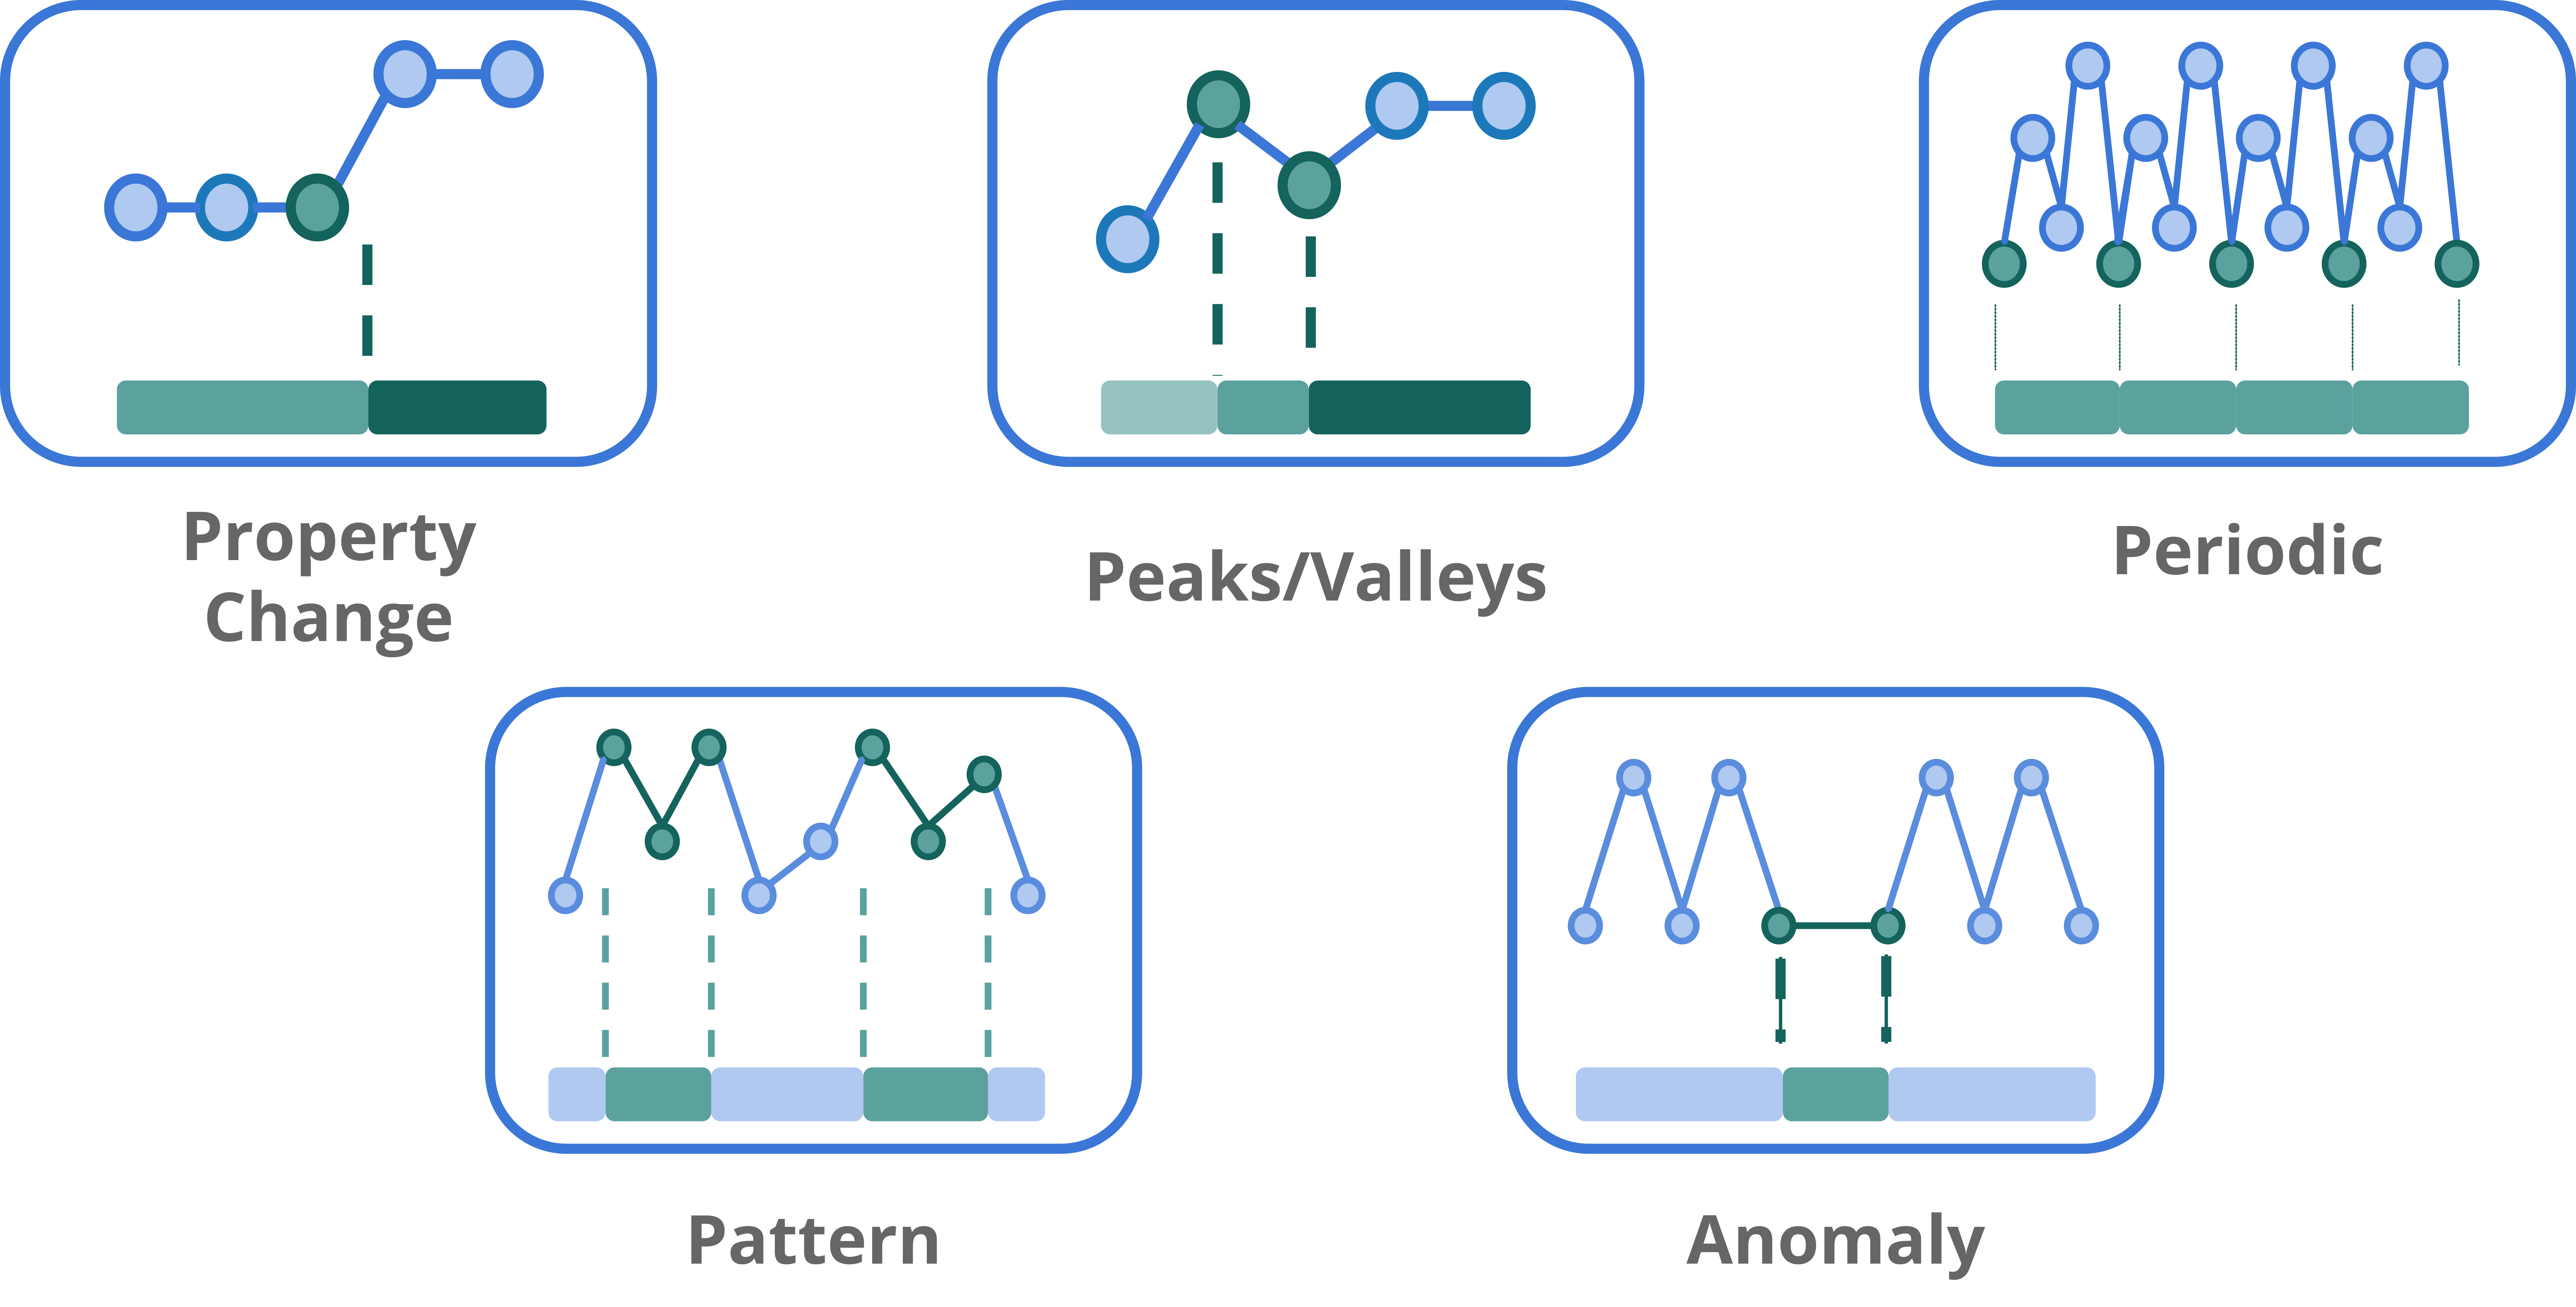
\includegraphics[width=0.95\linewidth]{event_type.png}
	\label{fig:event_search}
	\caption{}
\end{subfigure}
\caption{(a) Categories of search of events. In this case are shown Dimension, Window and Domain. (b) Examples of different type of events that can be considered significant in a time series.}
\end{figure}

Figures \ref{fig:event_search} and \ref{fig:event_type} are an illustrated summary of the two dimensions of the problem. Regarding the \textit{search} dimension, it is formed by three layers: \textit{(1) dimensionality}: the search can be made in one or multiple time series. In the multidimensional space, events can occur simultaneously in several time series, but other events can be specific for each of them (e.g. an accelerometer signal has 3 dimensions, but some gestures might be noticeable in only one of them); \textit{(2) time scale}: \textit{events} might occur in different time scales (e.g. when looking in a \textit{TS} of 1 hour long, we might see some relevant events, but when looking for a \textit{subsequence} of 10 minutes (zooming-in), other events are revealed); \textit{(3) domain}: the search procedure might be made directly on the time series by means of time properties, a distance measure (e.g. Euclidean distance), or can be made on the representation level, such as the feature domain.

\subsection{Type Dimension}

In what regards the \textit{event} type, we show in Figure \ref{fig:event_type} examples of events that are considered significant in a time series: \textit{(1) Property change:} when the change of a property or set of properties is greater than a threshold, such as changes on the mean (FIND THUMBNAIL IMAGE) or frequency (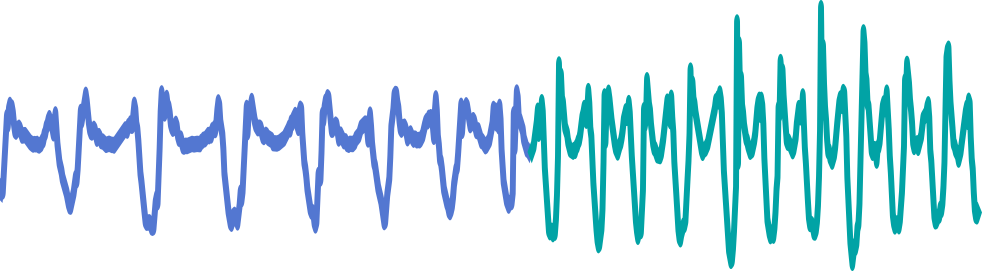
\includegraphics[height=3.5ex, valign=m]{walking_jogging.png}), \textit{(2) Peak/Valley}: peaks and valleys can typically be associated with significant physical changes (e.g. the peaks of an ECG signal 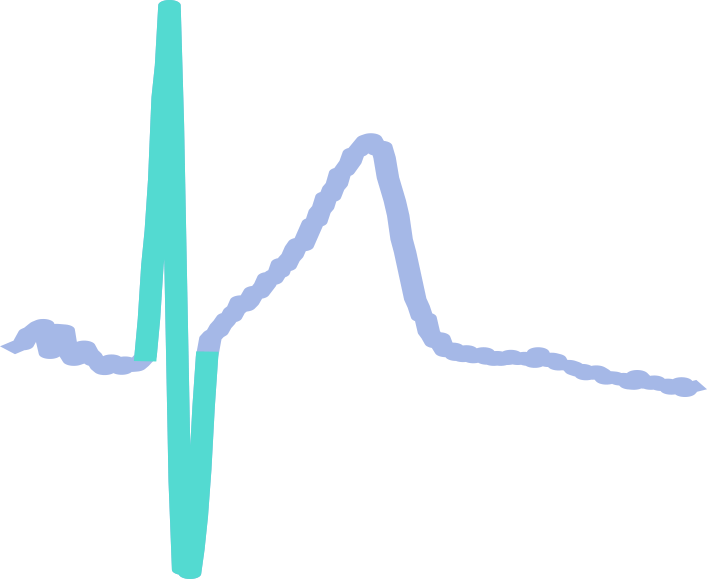
\includegraphics[height=3.5ex, valign=m]{high_peak_ecg.png}), \textit{(3) Periodicity}: if a signal is periodic, the moment each period starts is considered relevant (e.g. the cycles of a BVP signal 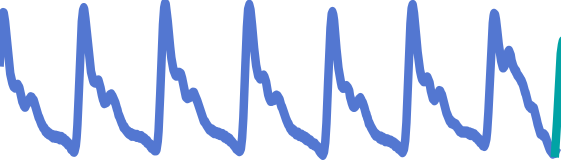
\includegraphics[height=2.5ex, valign=m]{bvp_segment.png}), \textit{(4) recurrent pattern}: re-occurrences of similar \textit{subsequences} with a certain shape or \textit{(5) anomaly}: very dissimilar \textit{subsequences} are relevant to indicate (e.g. noise in a clean signal 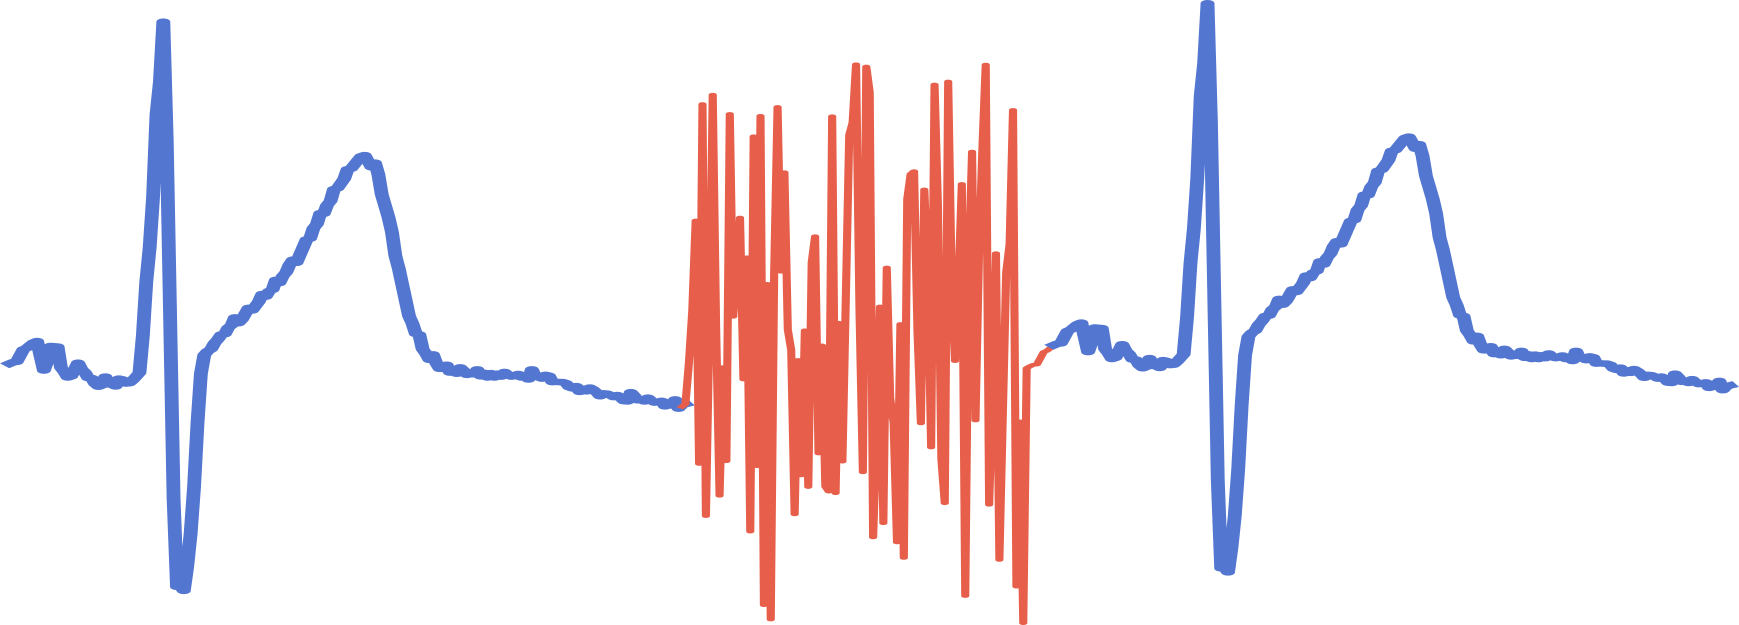
\includegraphics[height=3ex, valign=m]{ecg_noise_thumbnail.png}).

\subsection{Proposal}

In order to fill as much ground as possible in this problematic, we started by defining the search space considering that if the time series would be transformed in the feature space, any change in any of the features would be relevant, for instance, we might be searching for changes in the mean, standard deviation, mean frequency or other property. By characterizing the signal into the feature space, we are able to explore changes in all feature representations. Additionally, an event should separate two different behaviors. The notion of \textit{difference} in time series can be associated with \textit{distance/similarity}. This would enable to find change points, recurrent patterns, anomalies and periodic shapes. 
\par
Therefore, we propose an unsupervised methodology that searches for events in (1) uni and multi dimensional space, (2) with a fixed time scale, but with potential to be used in multi-time scale and (3) on a \gls{SSM} computed by a feature space representation of the time series. The events that will be searched are any relevant change in the matrix related with a change point and/or periodic event.
\par
We provide evidence that the proposed method is reliable for the detection of the mentioned events, supporting our claims with several examples in multiple time series domains (it is type agnostic) and comparing the results with state-of-the-art methods. Besides, we highlight that these events are all extracted from the same source of information (\textit{SSM}), while also providing some insights in how this could be expanded for multi-time scale search, used for summarization and labelling.
    
%IMPORTANT
%Besides, at the feature level, we are able to very easily include the information of \textit{MTS}. The fact that features can be used for this purpose might help in targeting and fine tuning the selection of features that work better for specific types of events or work domains (e.g. we might only be interested in changes related with frequency and not mean fluctuations, therefore, frequency features should be chosen, making targeted event search).

%Tools: Annotation, Segmentation, One-click segmentation of periodic events, summarization and profiling

\section{Building the SSM}

In this section, we explain the steps of the proposed method. The extraction of relevant events from time series starts by computing the \gls{SSM}. As explained in Chapter \ref{subsec:dist_matrix}, this matrix has relevant structural information to retrieve \textit{events}, namely \textit{blocks} and \textit{paths}. Figure \ref{fig:SSM_scheme} summarizes the steps involved in calculating the \gls{SSM}.

\begin{figure}
\centering
    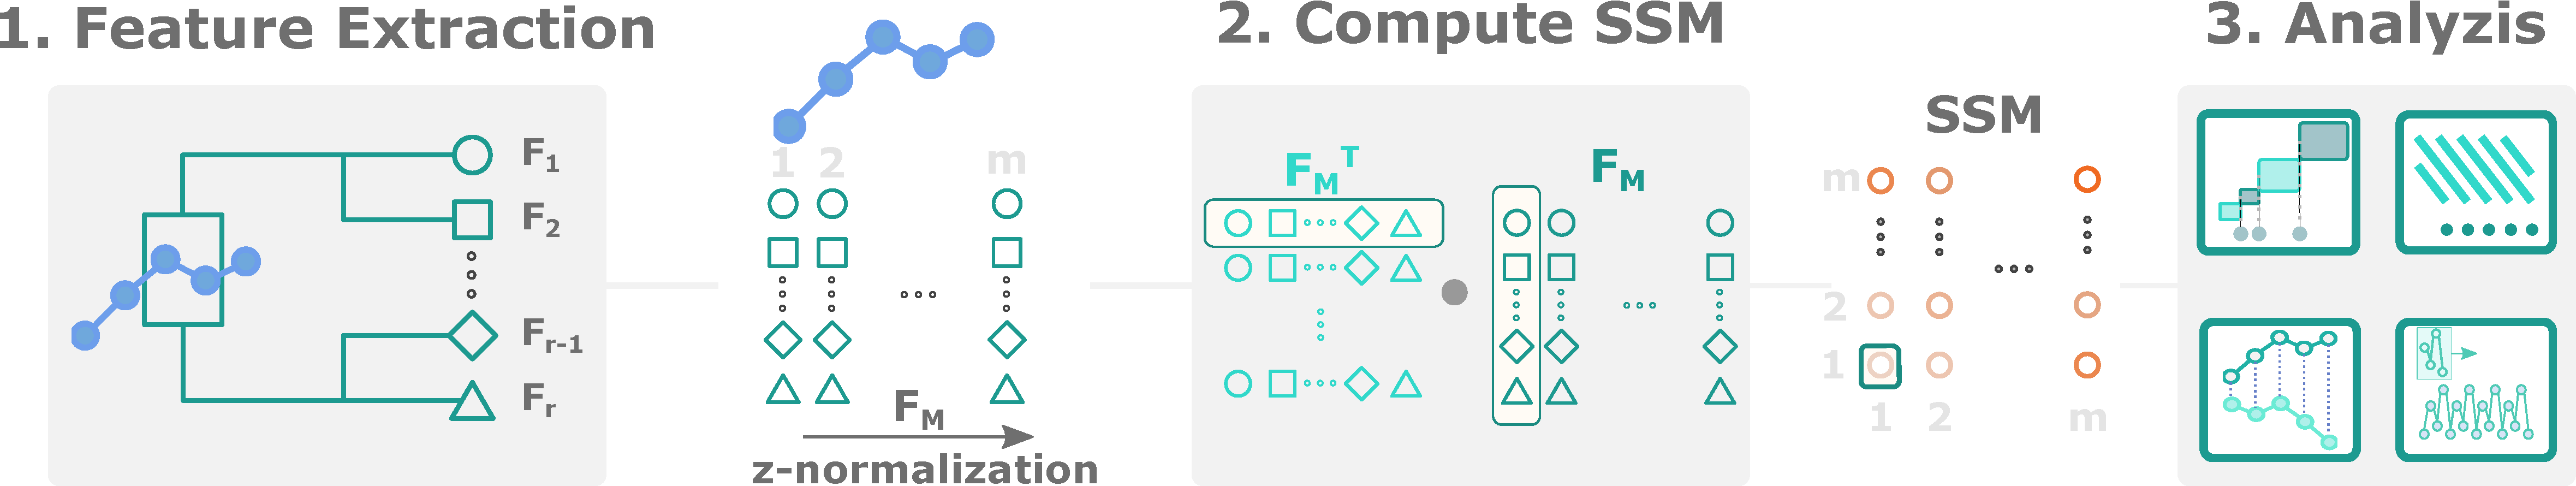
\includegraphics[width=\linewidth]{SSM_steps.pdf}
    \caption{Main process to reach the \gls{SSM}. The information needed to calculate the \gls{SSM} are the record and the input parameters: the window size (w) and the overlapping percentage (o). The first stage involves the feature extraction process, based on \textit{w} and \textit{o} values. Features are extracted on each window (1, 2..., N), being N the total number of windows. From the first window ($w_1$), are extracted features (f1, f2..., $f_K$, being \textit{K} the number of features used. The feature number is also associated with a shape (circle, triangle, etc...). The features can be extracted on multivariate records, being \textit{M} the number of records used. Each feature is positioned as a row on the $F_M$. Then follows the \gls{SSM} computation.}
    \label{fig:SSM_scheme}
\end{figure}

\subsection{Feature Extraction}

The structural information present on the SSM depends on the richness of the set of features into translating the changes and disruptions of the signal. Behavioral changes might be related with a variate set of features. As a feature may be sensitive for a type of change, the type of features should be diverse to identify a multivariate set of events and scan all types of signals. For this purpose, we used the available features from the TSFEL~\cite{barandas_tsfel_2020} Python library presented in the Feature Table \textbf{xxxx}.
\par
The features are extracted in a moving window with a size $w$, specified by the user, with an overlap of size $o$. These two parameters have a large influence on the results. The first defines the time scale at which features are extracted, therefore the wider the window, the more \textit{zoomed-out} will be the search. The second parameter defines the pixel-resolution of the resulting feature series, decreasing the amount of information (down-sampling) with a smaller overlap.
\par
The extracted features are grouped into a feature matrix ($F_{M}$), where the rows represent each feature and the columns the corresponding \textit{subsequence}, described by all features. Features extracted from a multidimensional record are ordered in the $F_M$ as rows as well. The total number of rows can be, at maximum: $r \times k$, being \textit{k} the number of time series being analyzed and \textit{r} the number of features extracted, as illustrated in Figure \ref{fig:SSM_scheme}.

\subsection{Feature-based Self Similarity Matrix}
\label{sec:the_ssm}

After grouping all the features extracted, the next stage applies a distance measure to the feature space and computes the \gls{SSM}. This process consists in comparing each \textit{subsequence} with the all the others within the time series record. Since each column of the $F_M$ is the feature characterization of each \textit{subsequence} by the entire set of features, the comparison between segments is achieved by calculating the dot product between the z-normalized transposed $F_{M}$ and itself:

\begin{equation}
    SSM = F^T_M F_M
\end{equation}

The dot product gives a similarity score based on the feature values of each \textit{subsequence}. Cells of the \gls{SSM} with higher similarity scores indicate that the corresponding \textit{subsequences} have similar feature values \cite{audiolabs1, audiolabs2}. As a result, the \gls{SSM} provides rich visual information, highlighting structures, such as blocks and paths, that describe the signal's morphological behavior over time and its structure.
\par

\begin{figure}
    \centering
    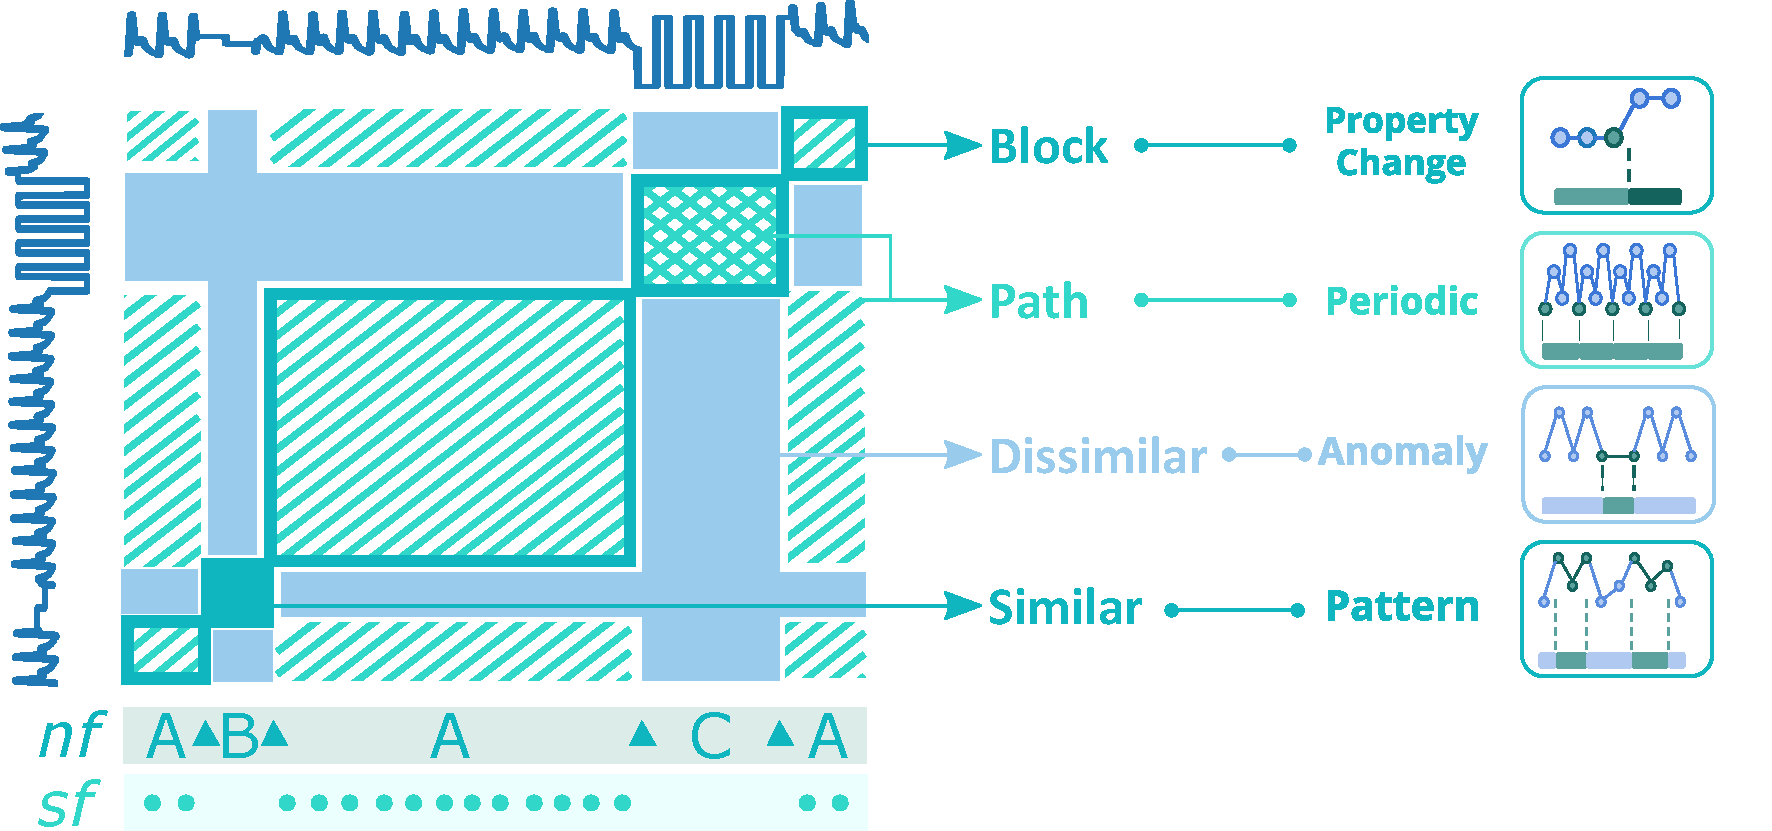
\includegraphics[width=\linewidth]{SSM_example.pdf}
    \caption{Description of informative structures of the \textit{SSM}. Based on the \gls{SSM} presented in Figure \ref{fig:first_image}, we show a simplified view with highlights on the relevant structures. The record has 4 main structures: A - homogeneous segment, which corresponds to the BVP periodic signal; B - homogeneous segment of missed data; C - homogeneous segment with detachment of the sensor. The boxes (blue) highlight homogeneous blocks while the sub-diagonals (orange) highlight periodicity in the segment. \textit{nf} and \textit{sf} indicate that the novelty and similarity functions are computed based on this information. Segment C has a cross-pattern, which indicates periodicity and symmetry}. 
    \label{fig:ssm_description}
\end{figure}

In Figure \ref{fig:ssm_description}, the main structures are illustrated and highlighted in an example of an \textit{\gls{SSM}} \cite{audiolabs1}. These structures are illustrated on the time series of example 1 (Figure \ref{fig:cold_start}. As mentioned in Chapter \ref{cha:methods1}, the main structures are \textit{blocks} and \textit{paths}. Our proposed methods for annotation takes advantage of these main structures to extract the desired information.
\par
\textit{Paths} show recurrence of patterns, which is an indication of matching the morphology between corresponding \textit{subsequences}. The example highlights circles in the \textit{sf} layer, indicating recurrence. In \textit{block} "C" are also visible \textit{inverse-paths}, which indicate symmetry, which means that the corresponding \textit{subsequences} are similar in reverse. The cross-path in \textit{block} "C" means that the \textit{subsequences} are periodic and symmetric.
\par
Differently, \textit{blocks} are square shaped structure that indicate homogeneous areas of the \gls{SSM}, which translate as constant behavior in the time series. The change between block structures along the main diagonal indicates a relevant change of morphology and behavior on the time series. In Figure \ref{fig:ssm_description}, the \gls{SSM} is segmented into several blocks on layer \textit{nf}. The triangular shapes indicate the change point that separate blocks "A", "B" and "C". Besides \textit{paths} and \textit{blocks}, the \gls{SSM} provides distance measures between \textit{subsequences}, which can be used to highlight dissimilar segments, such as anomalies or highlight very similar \textit{subsequences}, such as motifs (pattern).
\par
Several strategies were applied on the \gls{SSM} to extract the mentioned information. Further are explained the approaches used.

\section{Information Retrieval}

The \gls{SSM} is a powerful visual tool \textit{per se}, highlighting relevant information that could be missed if looking at the raw time series. However, being the information on the \gls{SSM}, it should be possible to retrieve it automatically. As Figure \ref{fig:info_retrieval_topics}, here are explained how to extract three layers of information, namely (1) change points in a time series (\textit{block} transitions), (2) periodic segmentation of patterns (\textit{paths}) and (3) how similar are the \textit{subsequences} segmented by the previous methods (\textit{distance profiles}). In addition, we will also demonstrate how the \gls{SSM} can be used to search queries in a periodic time series.

\begin{figure}
\centering

\includegraphics[width=\linewidth]{information_retrieval_topics.pdf}
\caption{Information retrieval topics explained in this section.}
\label{fig:info_retrieval_topics}
\end{figure}


\subsection{Novelty Search}

The search for \textit{novelty} is inspired by a method used in musical structure analysis and presented by \textit{Foote et al.} \cite{foote2000}. The process involves searching for transitions between \textit{blocks} using a moving checkerboard square matrix. The result is a 1 dimensional function designated \textit{novelty function} - \textit{nova}.
\par
As showed on Figure \ref{fig:kernel_description}, block transitions along the diagonal are represented by a checkerboard pattern. Detecting such patterns can be made by correlating a standard checkerboard matrix with the diagonal of the \gls{SSM}. For this, a sliding squared matrix, designated \textit{kernel}, is used. As illustrated in Figure \ref{fig:kernel_shape}, the kernel has a checkerboard pattern and is combined with a Gaussian function to add a smoothing factor. The kernel, $K_N$, is a combination of two different kernels: $K_H$ and $K_C$. The first is responsible for identifying the homogeneity of the \gls{SSM} in each side of the center point along the diagonal. The higher the homogeneity, the higher will be the values in these sections. The latter measures the level of cross-similarity, returning higher values in cases of high cross-similarity. Therefore, when sliding the kernel $K_N$ along the diagonal, a higher correlation value will be returned when it reaches a segment of the \gls{SSM} with a similar checkerboard pattern. The result is the mentioned $nova$ \cite{Dannenberg2008, Mueller15_FMP_SPRINGER, MuellerZ19_FMP_ISMIR}.

\begin{figure}
    \centering
    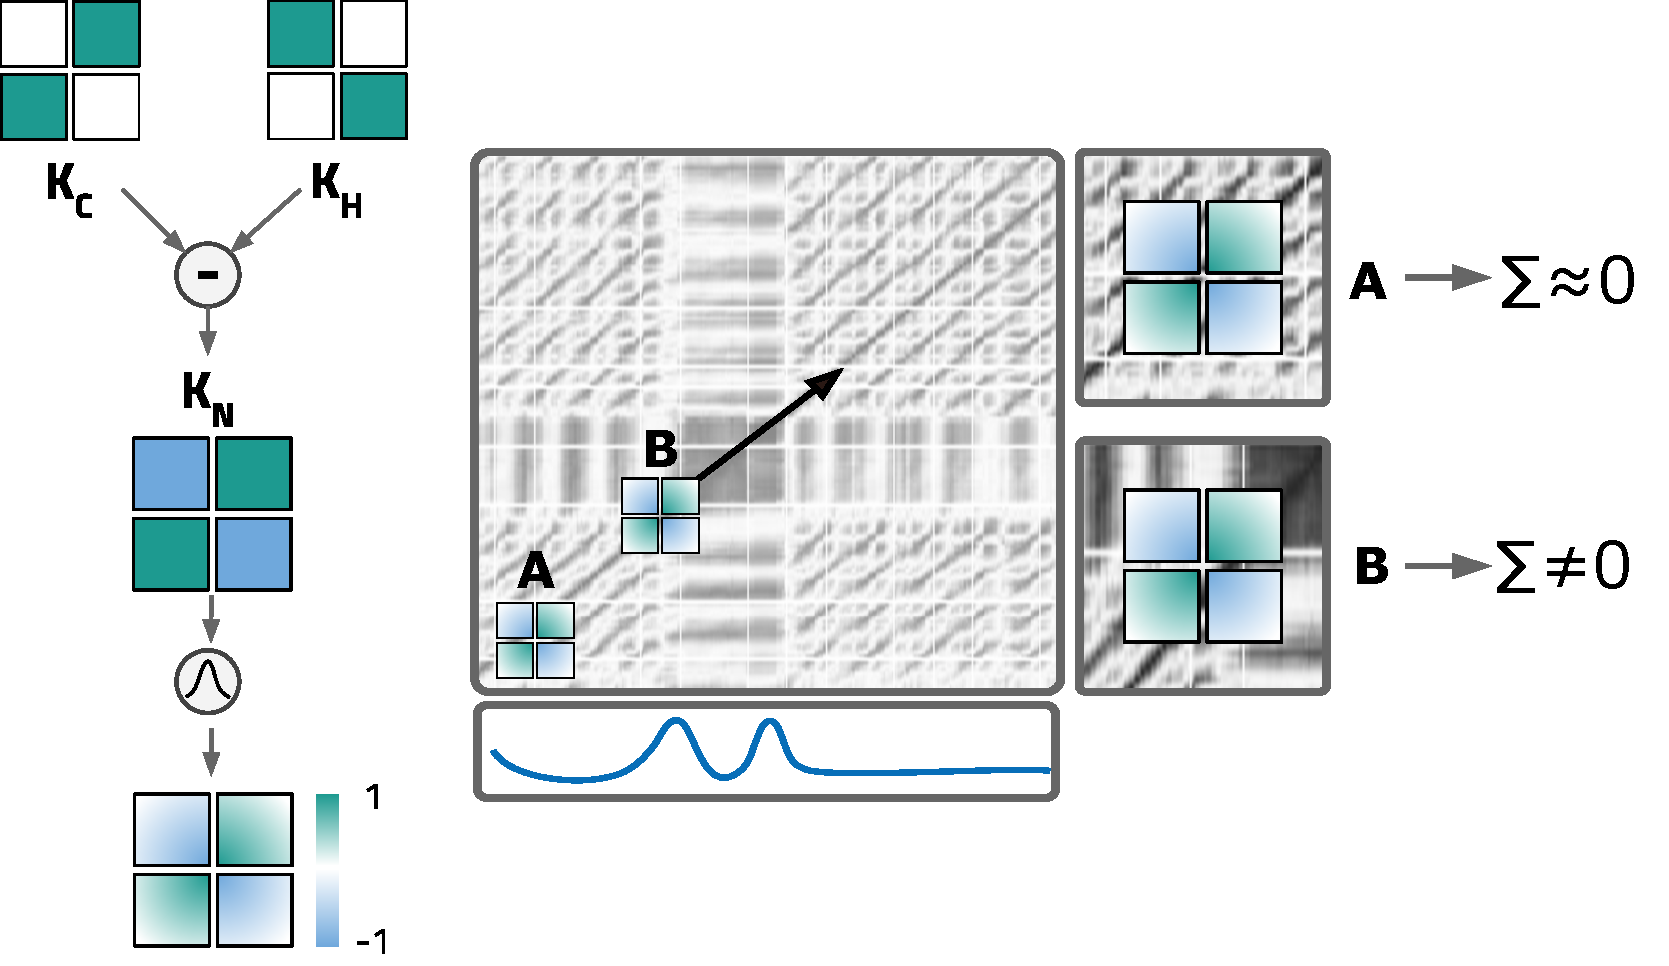
\includegraphics[width=\linewidth]{kernel_sliding.pdf}
    \caption{(left) Description of the matrix (kernel) used to compute the \textit{novelty function}. The checkerboard pattern is achieved by combining kernel $K_H$ - measure of homogeneity; and $K_C$ - measure of cross-similarity. The resulting kernel ($K_N$) is combined with a Gaussian function to generate $K_G$. The Figure is based on the works of \textit{Mueller et al.} \cite{Mueller15_FMP_SPRINGER, MuellerZ19_FMP_ISMIR}; (right) The process to compute the novelty function is described. Kernel $K_G$ is slided along the diagonal of the \gls{SSM} to compute the \textit{novelty function} presented as the bottom sub-plot. Positions A and B show the effect of block transitions on the \textit{novelty function}. Figure based on the works of \cite{Dannenberg2008, Mueller15_FMP_SPRINGER, MuellerZ19_FMP_ISMIR}.}
    \label{fig:kernel_description}
\end{figure}

As showed in Figure \ref{fig:kernel_description} (left), the kernel in position \textbf{A}, which is placed on an area of high homogeneity, returns a value close to $0$ when summing the product between it and the section of the \gls{SSM} it overlaps. In the other end, in position \textbf{B}, the kernel reaches a segment with low cross-similarity and high diagonal similarity, which results in high correlation values with a checkerboard pattern. The \textit{nova} is high in these transition segments \cite{Dannenberg2008, Mueller15_FMP_SPRINGER, MuellerZ19_FMP_ISMIR}.
\par
Each section of the kernel has the same size, \textit{L}, being the total kernel size configured by $D = 2 \times L + 1$, with $L \in \mathbb{N}$ . The kernel has an odd size to adapt zero values in centered points. It also has total size D $\times$ D, being $K_{N}$ defined by the following function \cite{Mueller15_FMP_SPRINGER, MuellerZ19_FMP_ISMIR}:

\begin{equation}
        K_N(i,j)  = \sgn(a_i) \cdot \sgn(b_j)
\end{equation}

being $a, b \in [-L:L]$ and "\sgn" representing the sign function, which indicates the sign of the value (1, 0 or -1). A radially symmetric Gaussian function is used to smooth the Kernel, with the following equation \cite{Mueller15_FMP_SPRINGER, MuellerZ19_FMP_ISMIR}:

\begin{equation}
    \phi(p,u) = \exp(-\frac{1}{2L\sigma^2}(p^2 + u^2))
\end{equation}

being $\sigma$ the standard deviation, equal for both $x$ and $y$ dimensions of the matrix, $L$ the size of each kernel's section, and $p$ and $u$ the position in the $x$ and $y$ dimensions, respectively. The final kernel is computed by point-wise multiplication with the Gaussian function:

\begin{equation}
    K_{G} = \phi \cdot K_{N}    
\end{equation}

The \textit{nova} is calculated by correlating the kernel with the diagonal of the matrix:

\begin{equation}
    nova(m) = \sum^{2L+1}_{i,j=0} K_{G}(a_i,b_j)SSM(m+a_i, m+b_j)
\end{equation}

being the sample of the novelty function $m \in [0-N]$ and $a, b \in [-L:L]$. The change point events are represented by local maxima (peaks) in \textit{nova}, which can be detected by standard peak finding strategies.

\subsection{Periodic Search}

As aforementioned, \textit{paths} indicate the presence of similarity and reoccurring patterns can be visualized on the \gls{SSM}. The moment in time the \textit{paths} start indicates the position at which the period of the pattern begins. In order to find the periodicity, we compute the similarity function, $s_f$, which is calculated by summing the values of the $\gls{SSM}$ column-wise (either column-wise or row-wise would work, since the matrix is symmetric), being each element of the $sf$ calculated by:

\begin{equation}
sf(x) = \sum_{i=0}^{m}{SSM_{ix}}
\end{equation}

\noindent where \textit{i} is the column position for the sum, $sf_{j}$ the sample of the function at position \textit{j} and \textit{m} the size of one of the dimensions of the \gls{SSM}, which is equal to the feature-series size. As segments with similar morphology will be similarly described by the extracted features, the columns will have a similar representation, hence a similar value on the \textit{sf}. In cases where the time series is periodic, the similarity function will enhance this behavior by having valleys at the moment the \textit{path} starts. The identification of events related with the periodicity of a time series is then possible by searching for local minima (valleys) on the similarity function.  

\subsection{Similarity Profiles}

The main elements, \textit{blocks} and \textit{paths}, are essential sources of information for the segmentation of the time series. Besides these, the \gls{SSM} also provides the pairwise similarity values between all \textit{subsequences} of the time series. This is an important measure that gives an understanding of how close together are each \textit{subsequence} and can be used to cluster them. In order to use the similarity values of the \gls{SSM} to compare \textit{subsequences} we compute \textit{similarity profiles}.
\par
The comparison between \textit{subsequences} could be made by directly using the values of the matrix in the segment delimited by both \textit{subsequences}. Although this would be a legitimate process, we find that a stronger measure is to compare how much each of the two \textit{subsequences} are similar/different to all the other \textit{subsequences} of the time series. For this, \textit{similarity profiles} ($P_s(c)$) are computed as the average similarity values of a section of the \gls{SSM} delimited by the \textit{subsequence} being profiled, with size $w$,  and all the other \textit{subsequences} of the time series, with size $m$:


\begin{equation}
P_s(c) = \frac{\Sigma_{i=0}^w SSM(i, c)}{w}
\end{equation}

The \textit{similarity profile} is computed column-wise, being each column $c$ the average similarity value between the reference \textit{subsequence} and the \textit{subsequence} corresponding to $c$. The reasoning is that similar \textit{subsequences} should have closer \textit{similarity profiles}. Since the profiles have the same size, these can then be compared with the \textit{euclidean distance} and clustered based on these distance values. This process is specially valuable to cluster the segments previously extracted with the \textit{nova} and \textit{similarity} functions.

\begin{figure}
\centering
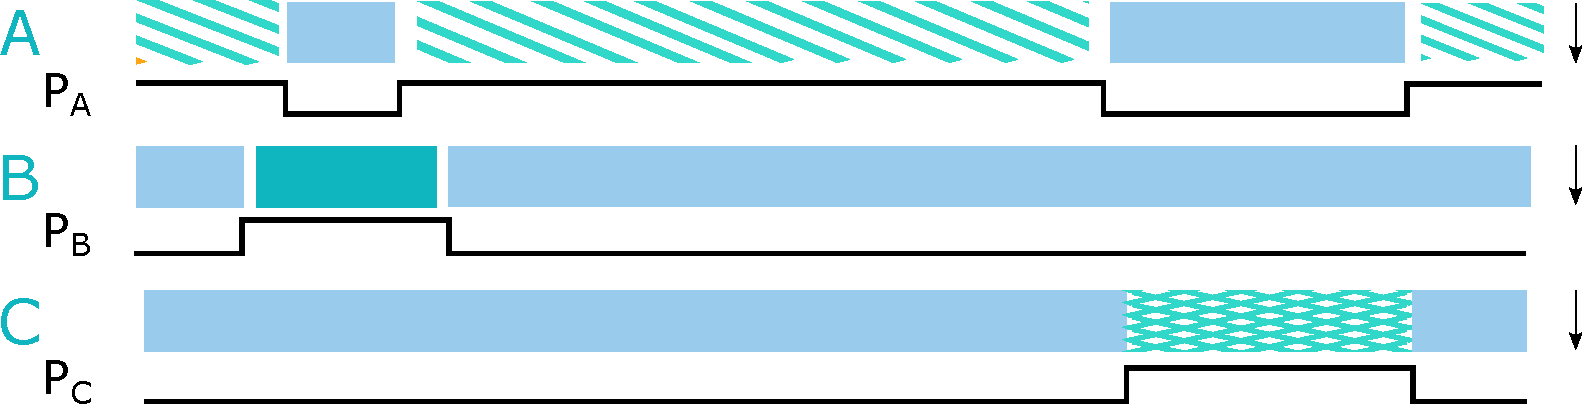
\includegraphics[width=\linewidth]{profiles.pdf}
\caption{Profiles computed for each segment of the example signal used in Figure \ref{fig:ssm_description}.}
\end{figure}

A general example of applying this process to the segmented time series based on the \textit{nova} function is showed in Figure \ref{fig:profiles}. Each segment category (A, B and C) extracted from the \gls{SSM} of Figure \ref{fig:ssm_description} is computed into a profile ($P_A$, $P_B$ and $P_C$) by averaging column-wise. These \textit{similarity profiles}show how similar the segment is with all the other \textit{subsequences} of the time series. All segments A will have a similar $P_A$, while being very different from profiles $P_B$ and $P_C$. 

\subsection{Query Search}

Another relevant application of the \gls{SSM} is to make query search based on examples. The process follows the traditional methods of template-based search methods explained in Chapter \ref{sec:query_based_search), but instead of doing the process directly on the time series, it is performed on the \gls{SSM}. The search procedure works by sliding the smaller column window (the example selected on the time series) along the \textit{SSM}, one sample at a time. The distance, $D$, between the example and the segment it slides over is calculated through the sum of absolute differences:

\begin{equation}
    D(i) = \sum_{i=0}^{i=m}{\sqrt{(SSM(i) - SSM_t)^2}}
\end{equation}

\noindent where $SSM(i)$ is the segment of the \textit{SSM} over which the example, $SSM_t$, slides at moment $i$, up to the size of the \gls{SSM}. The resulting distance function has minimums at the position where the example is matched.


\section{Experimental Evaluation in Selected Use-cases}

After explaining the process to represent the time series into a feature-based similarity matrix and the methods used to retrieve information from it, we present selected use-cases from multiple domains to exemplify its universal usage.

\subsection{Use-Case 1 - Human Activity}

\begin{figure}
    \centering
    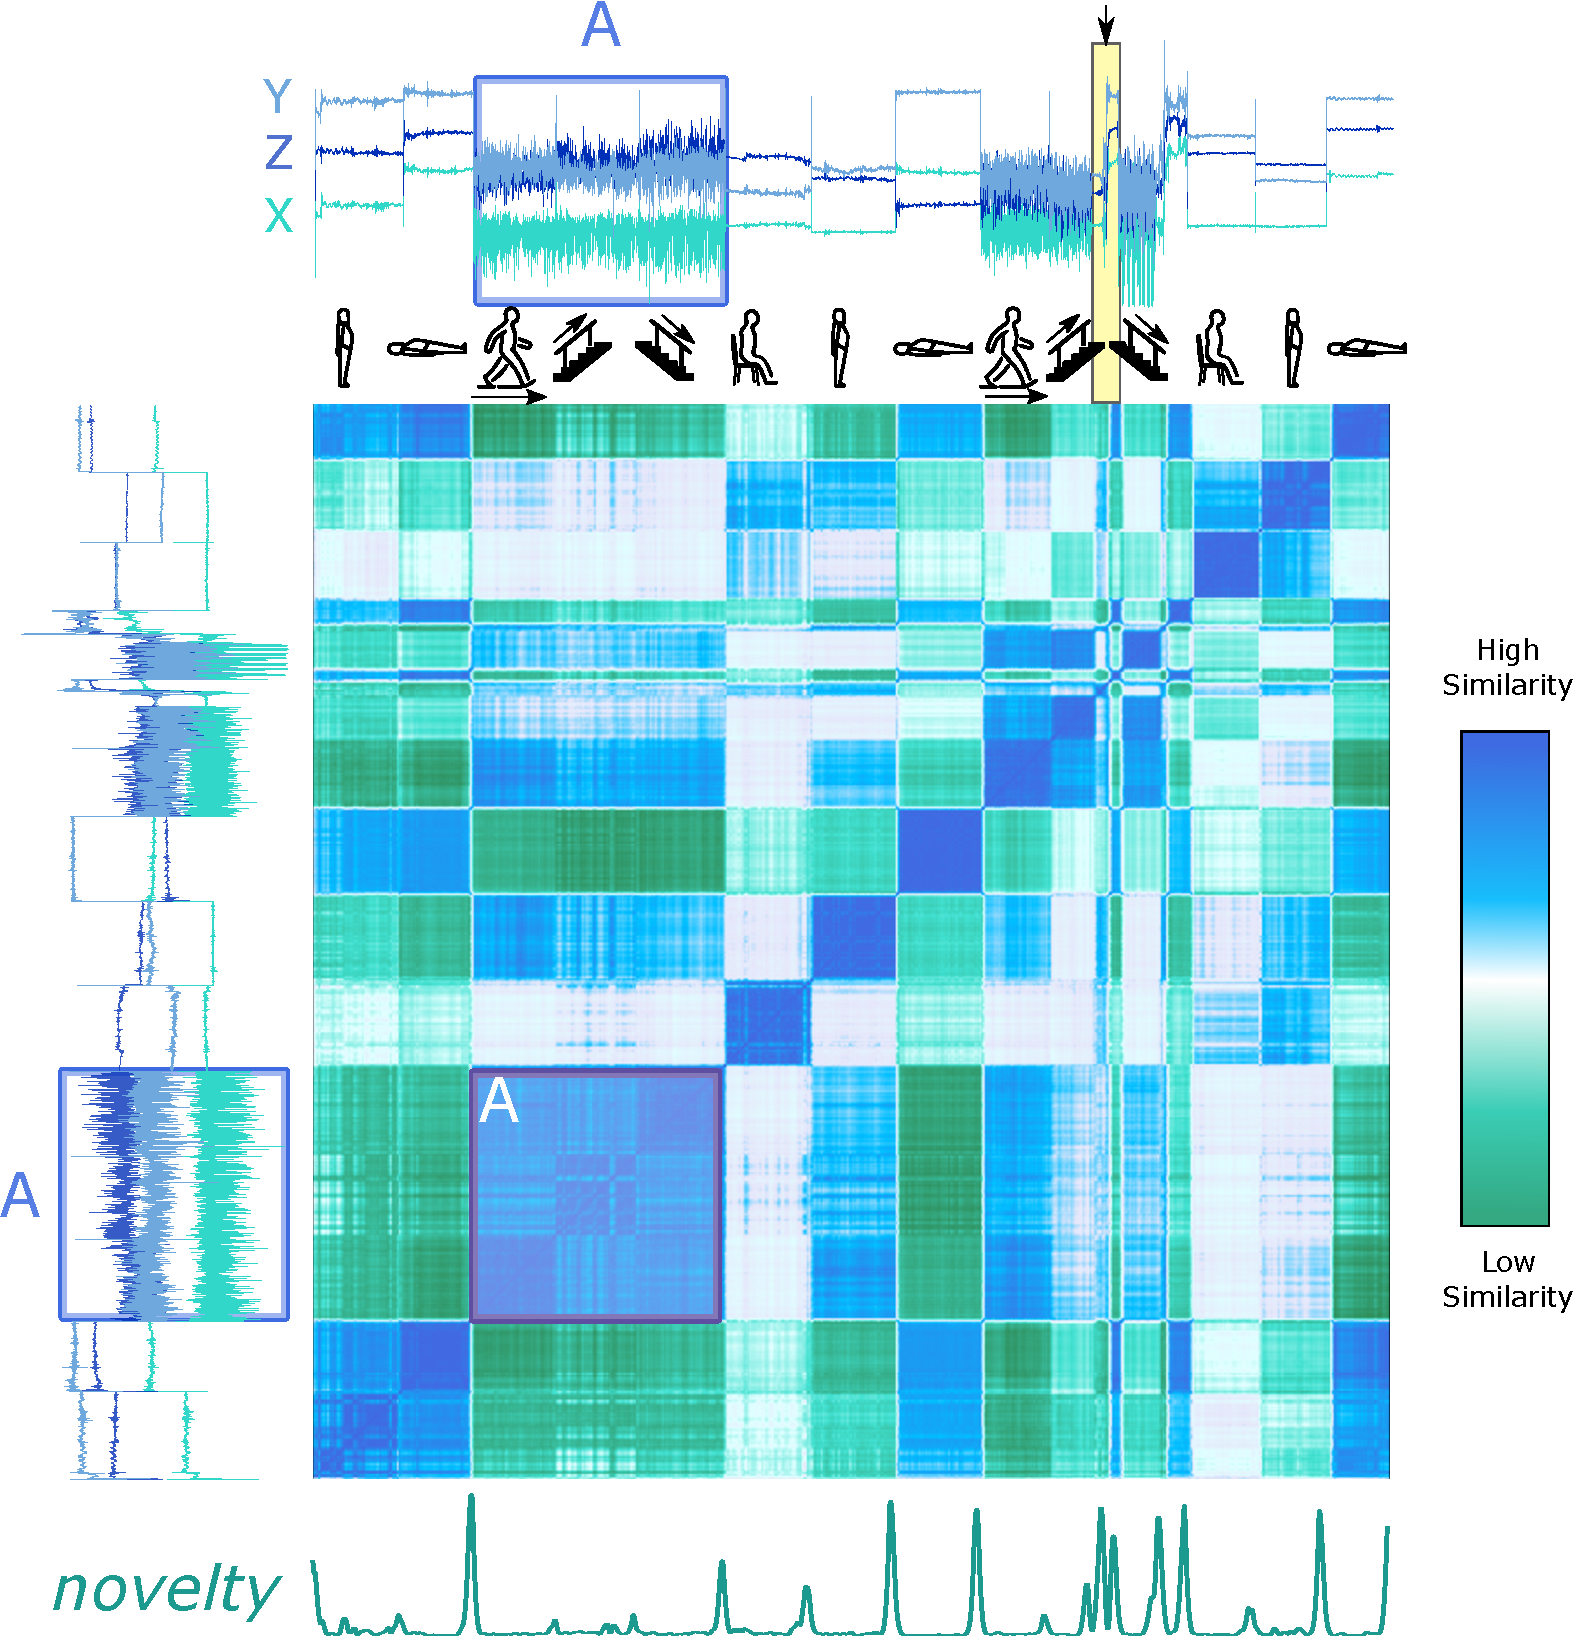
\includegraphics[width=\linewidth]{use_case1_HAR.pdf}
    \caption{Change point event detection strategy applied on the SSM to search for change point events. The sequence of activities is presented as follows: $Sitting \xrightarrow[]{} Laying \xrightarrow[]{} Walking \xrightarrow[]{} Upstairs \xrightarrow[]{} Downstairs \xrightarrow[]{} Sitting \xrightarrow[]{} Standing \xrightarrow[]{} Laying \xrightarrow[]{} Walking \xrightarrow[]{} Upstairs$. The input variables used are $time_{scale}$=250 samples, $kernel_{size}$=45 samples, overlap=95\%}
    \label{fig:use_case1}
\end{figure}

The example presented in Figure \ref{fig:event_search_demonstration} shows the usage of the \gls{SSM} on a record of Dataset 2. In this example, the method was applied to all the 3-axis of the accelerometer data. All are showed and described with the sequence of activities as captioned in Figure \ref{fig:use_case1}.
\par
The \gls{SSM} was computed using a window size of 250 samples, and an overlap of 95 \%. The color \textit{blue} indicates segments with higher similarity. Along the diagonal, these blocks are visible and the events are estimated as the transition between these, highlighted by the \textit{nova} function. The kernel used for this detection had a size of 45 samples.
\par
In this example, we can identify that the detected change point events match with the activity transitions. Although all transitions are visible on the novelty function, the ones that correspond to transitions between similar segments of activities are harder to find, namely the transitions between walking activities. This is plausible since the properties of these segments are similar and the morphological difference is not as significant as when shifting between dissimilar activities (e.g. between \textit{Laying} and \textit{Walking}).
\par
Any significant change in properties will be detected by the proposed method. As presented in Figure \ref{fig:event_search_dimension}, at the end of the time series, the period in which the subject was performing the \textit{Walking upstairs} activity is affected by other changes in the time series. These are significant and also correspond to \textit{block} transitions, which are also evident in the novelty function. The proposed strategy, being unsupervised, is sensitive to any change, as long as it is observed as a significant change in the signal's properties\\


\begin{figure}
    \centering
    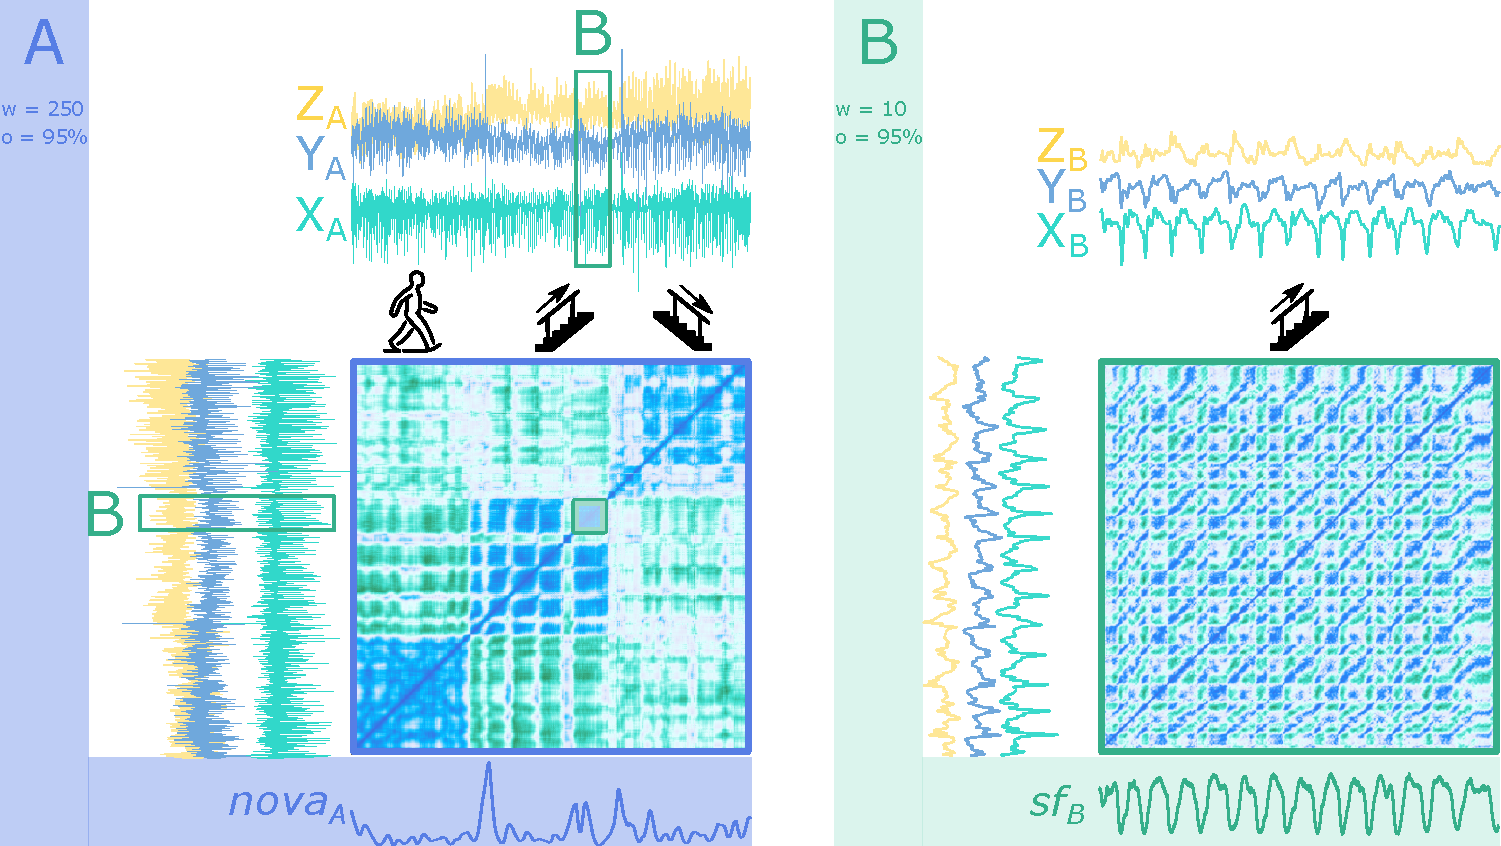
\includegraphics[width=\linewidth]{use_case1_HAR_zoom_in.pdf}
    \caption{ABP signal change point detection. The parameters used were a size of 5000 samples, with an overlap of 75\% and a kernel size of 25 samples.}
    \label{fig:example1_zoom}
\end{figure}

When \textit{zooming-in} the \textit{SSM} into segment \textit{A}, which shows transitions between walking behaviors, the checkerboard pattern that highlights change points is clearer and the three different walking patterns are easily segmented. The two major peaks in the corresponding \textit{nova} function are from these transitions, as presented in Figure \ref{fig:example1_zoom} (left). In addition, the reader might notice that the segments of the matrix related with \textit{walking in stairs} are also segmented into smaller \textit{blocks}. Although the information is not available on the dataset description, we strongly believe these are flight of stairs.
\par
Considering that the signal is a walking behavior, the reader might question the fact that the periodicity of the walking pattern is not exhibited on the matrix. The reason is that the window size used to compute the \gls{SSM} of Figure \ref{fig:use_case1} is too large. If features are extracted with a smaller window size, closer to the walking period, the \textit{paths} that indicate the recurrence of shapes are visible. Figure \ref{fig:example1_zoom} (right) shows the \gls{SSM} built from the segment \textit{B} of the original time series, with a window size of 10 samples and an overlap of 95 \%. The matrix shows the \textit{paths}, from which it is possible to extract the periods with the similarity function ($sf_B$).


\subsection{Use-Case 2 - Medical domain}

In the medical domain there are several examples of structural information to retrieve. Some signals are periodic, such as the \gls{ECG}, the \gls{ABP} or the \gls{RESP} signals. When acquiring this type of data, several instances might reflect unexpected changes, either because of physiological responses and medical disorders or due to the sensing process. Here we show two examples of physiological changes in two periodic signals.
\par
The \gls{ABP} signal can change due to postural changes. An experiment was conducted to study this effect and is available at Physionet \cite{tilt, PhysioNet}. In Figure \ref{fig:example2_3} is showed the process of segmenting the \gls{ABP} signal based on postural changes, signaled with the ground truth. The change points are well perceived by the proposed strategy. The reader can notice that the shape of the \gls{ABP} signal in each regime is very similar, being  hard to notice by human eye where it happened. In addition, the periodicity of the signal is not visible on the matrix because the features were extracted with a window size of 5000 samples, which is much larger than the size period length.
\par
The \gls{SSM} of Figure \ref{fig:example2_3}.a also shows which segments are similar to each other. The blue colors of the matrix indicate high similarity and it is clearly presenting that segments with positive \textit{posture change} are more similar.

\begin{figure}
    \centering
    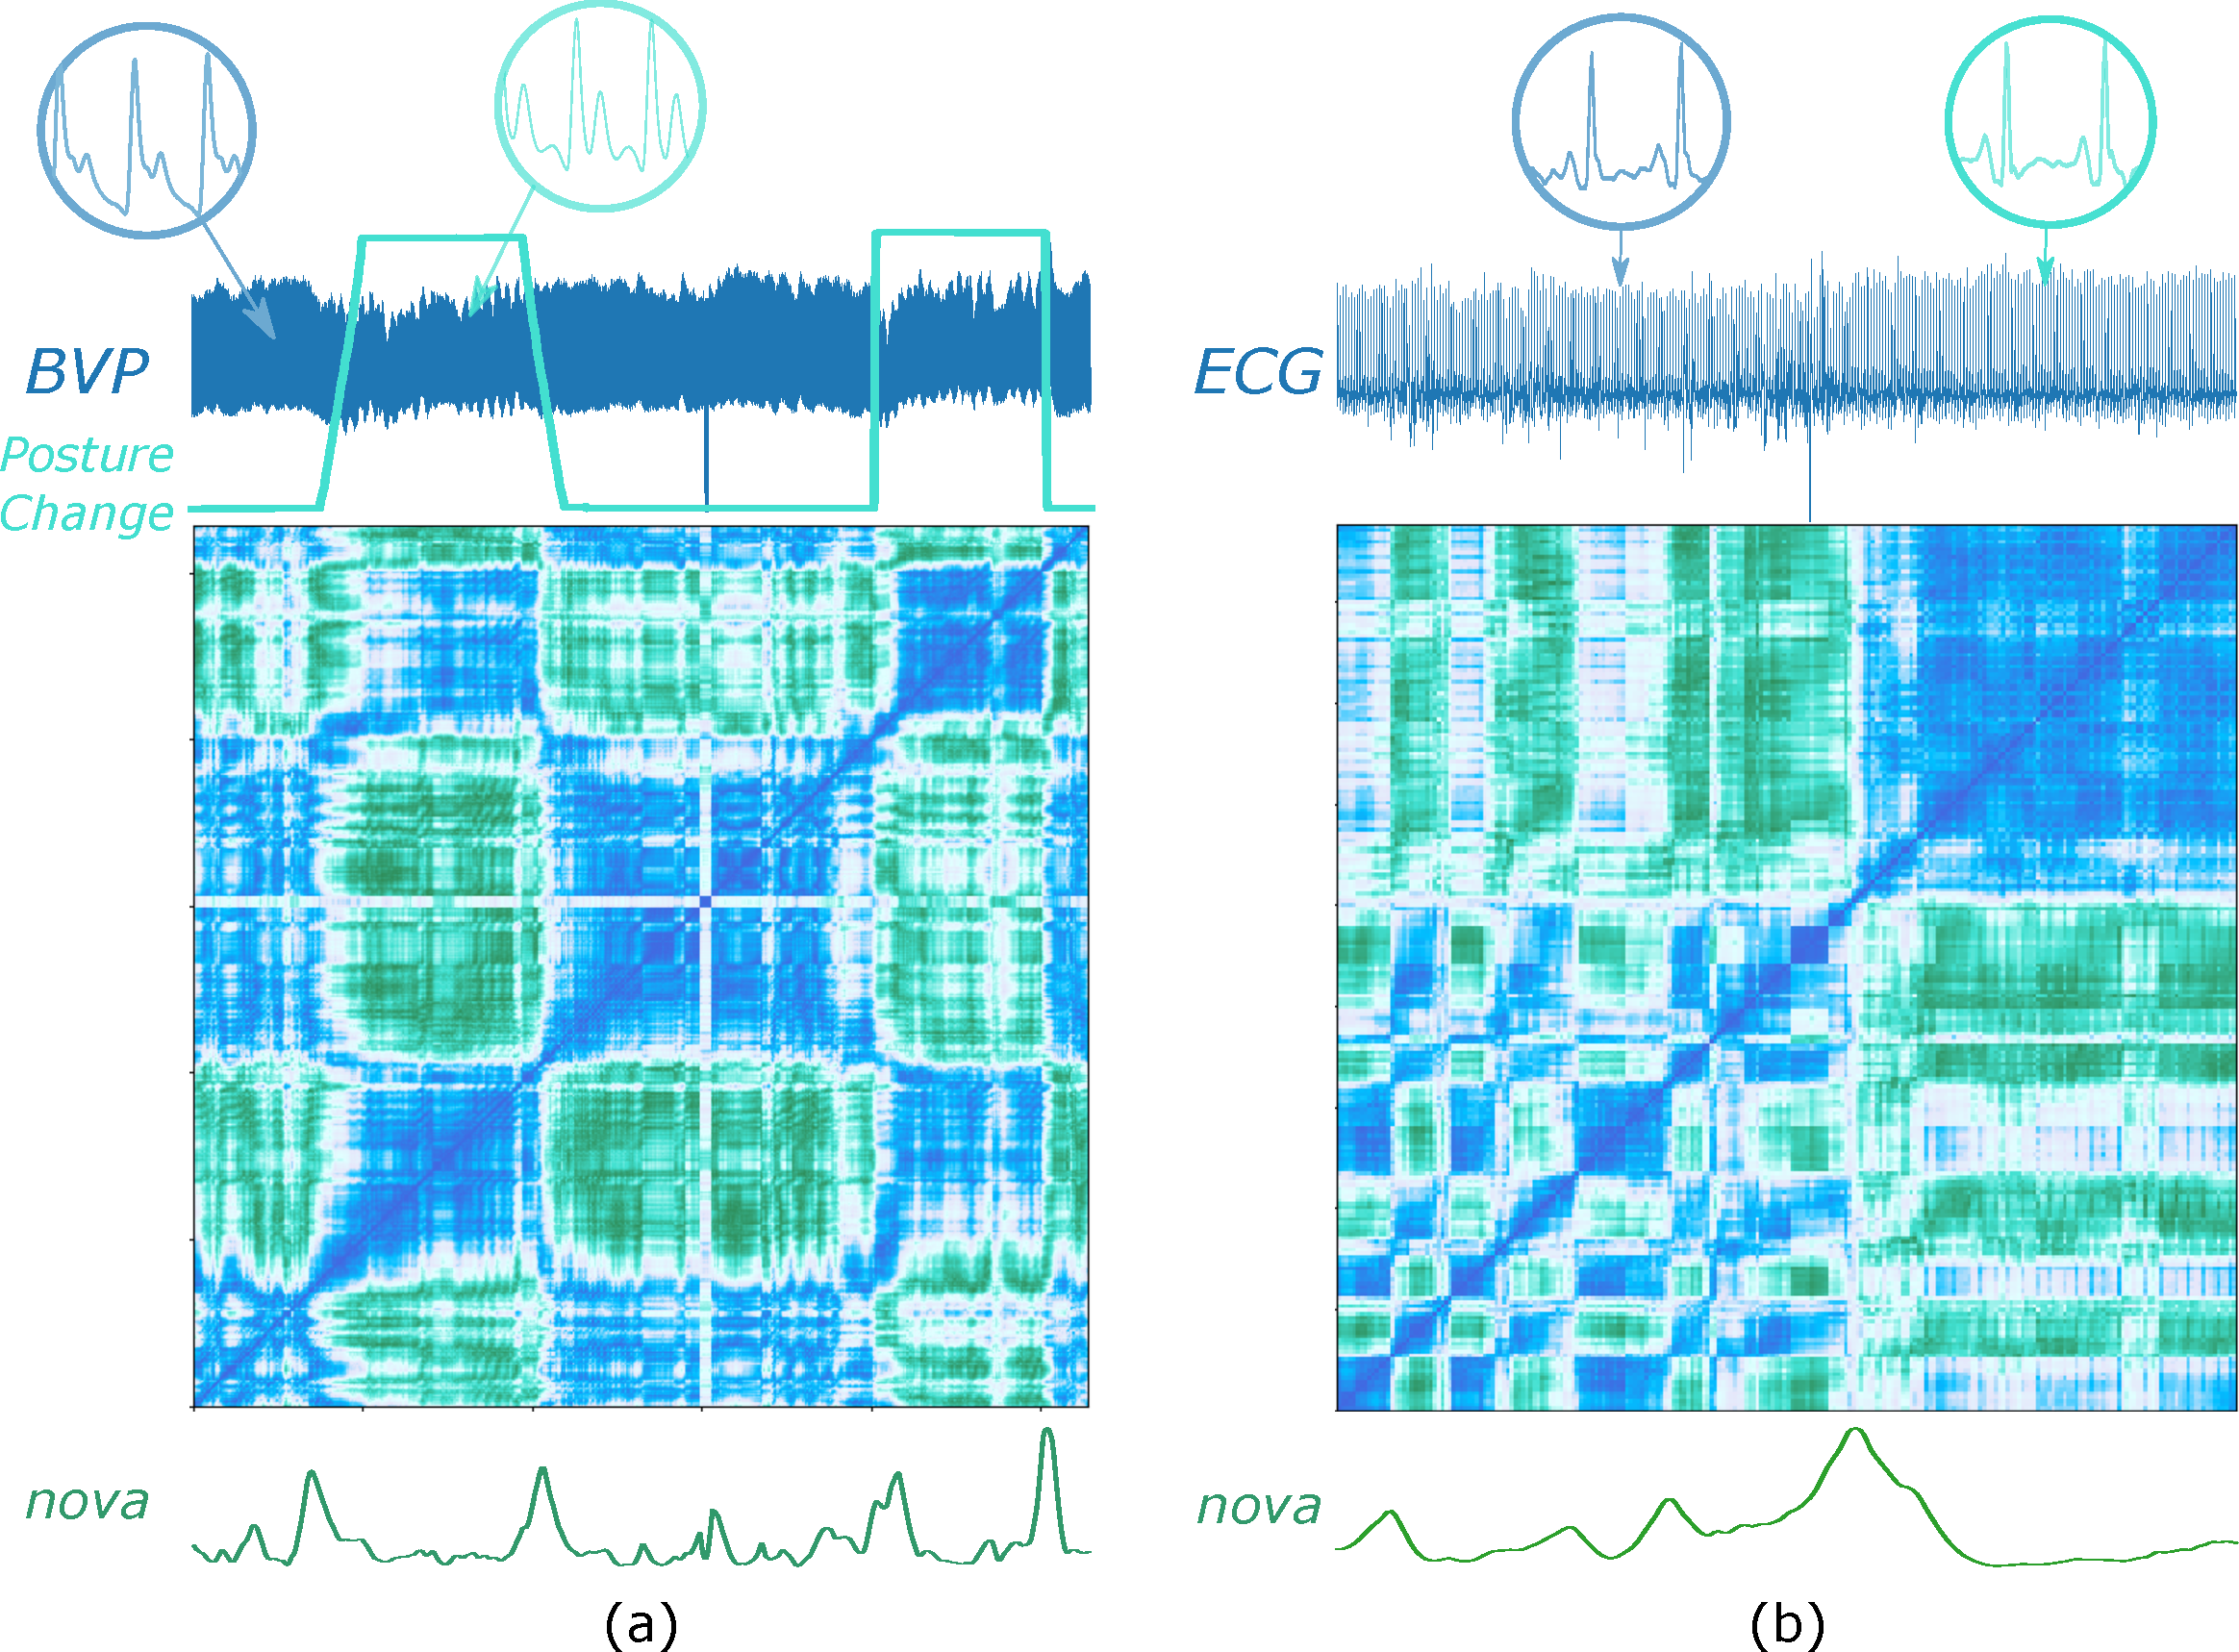
\includegraphics[width=0.9\linewidth]{use_case2and3_bvp_pulsus.pdf}
    \caption{(a) ABP signal change point detection. The parameters used were a size of 5000 samples, with an overlap of 95\% and a kernel size of 200 samples.}
    \label{fig:example2_3}
\end{figure}

The same happens on the \gls{ECG} signal from Figure \ref{fig:example2_3}.right. It displays a condition called pulsus paradoxus.... Again, the reader can notice that the change point is hardly perceivable by human eye, but the proposed strategy is able to clearly show the difference in both regimes.

\subsection{Use-case 3 - Multidimensional}

\begin{figure}
    \centering
    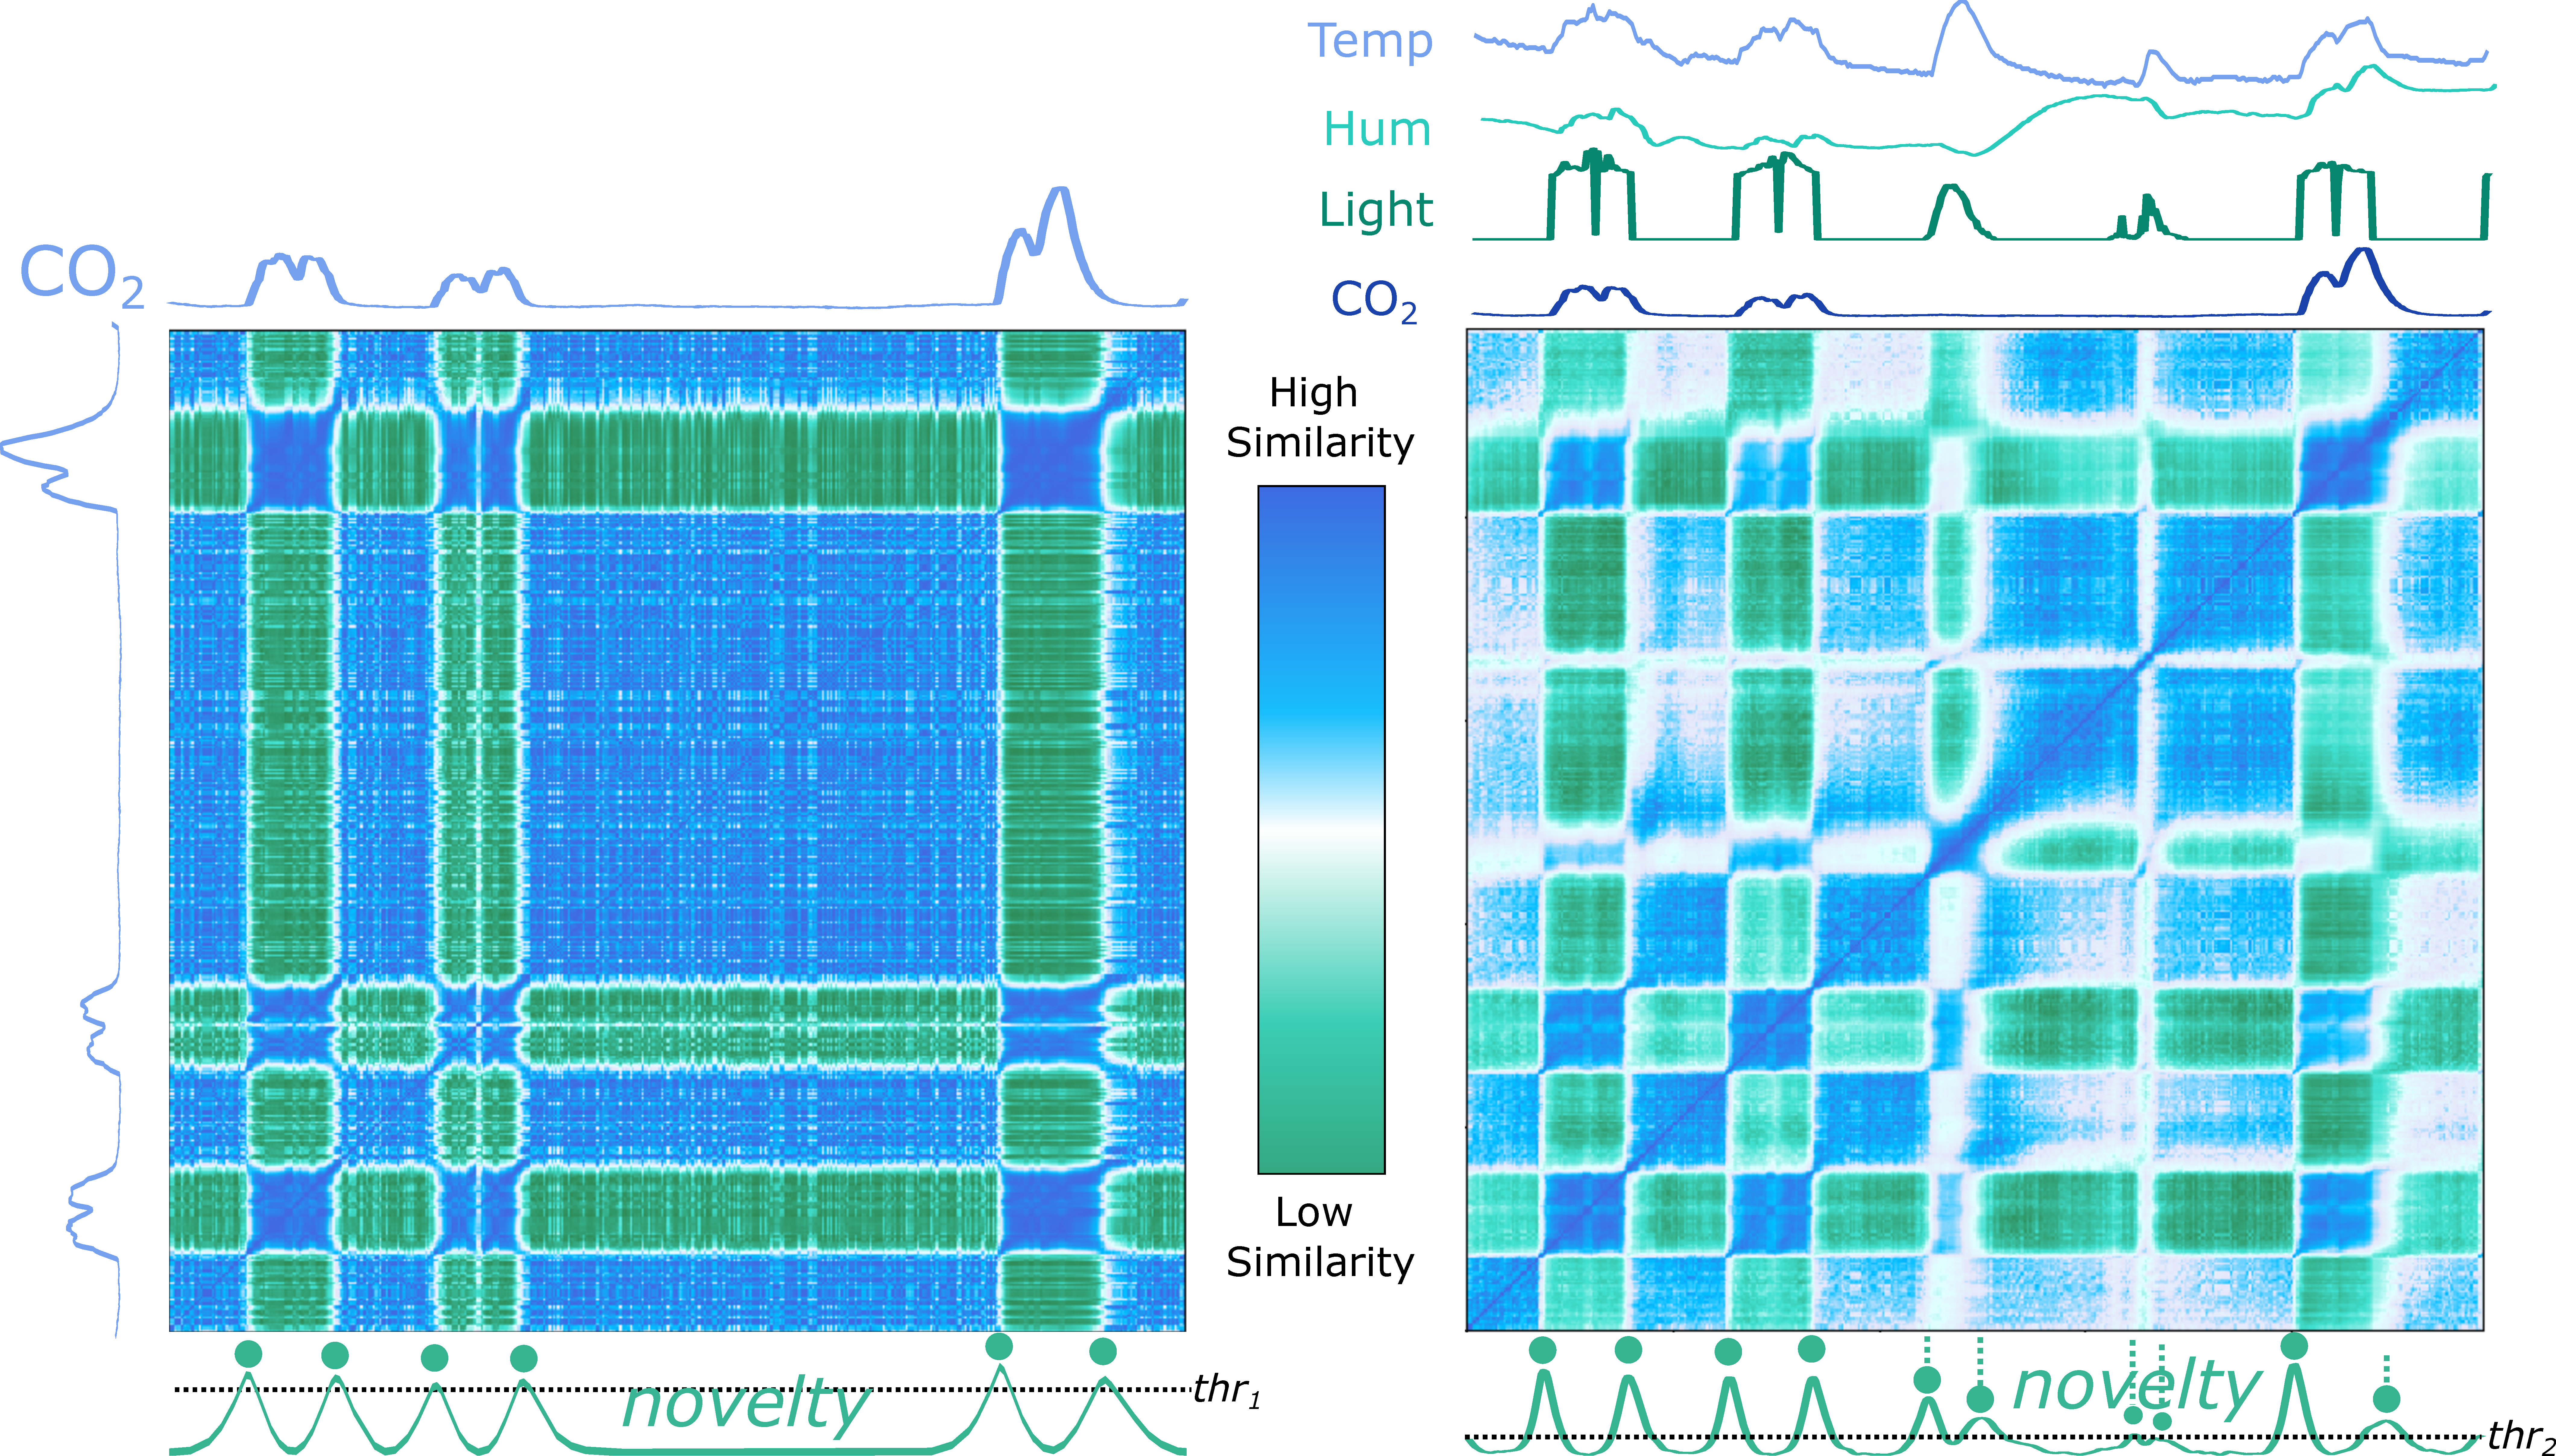
\includegraphics[width=0.9\linewidth]{use_case4_multi.pdf}
    \caption{Proposed method applied on "\textit{Occupancy}" record of Dataset \ref{sec:dataset8}. (a) A single time series of the record is used to extract events; while in (b) the \gls{SSM} is computed with features extracted from the four available time series.}
    \label{fig:example4}
\end{figure}

The proposed method accepts both single and multidimensional records. The difference regards the number of features extracted. As presented on Figure \ref{fig:SSM_scheme}, the same set of features are extracted for each time series of the record and combined in the $F_M$. 
\par
Using a single time series of a multivariate record is optional and depends on the detection's purpose. In some cases, using a single time series from a multidimensional record can lead to missing relevant events undetected. An example of this can be seen on Figure \ref{fig:example4}.a with record \textit{"Occupancy"} from Dataset \ref{sec:dataset8}. 
\par
The record is a multi-dimensional time series that measures room occupancy based on temperature, humidity, light and $CO_2$. All events can only be detected if using several time series of the record \cite{cpd_alan}. On Figure \ref{fig:example4}.a, a single time series was analyzed by the proposed method to detect relevant events, while Figure \ref{fig:example4}.b is the result of using all the time series of the record.

\section{Time Series Profiling}

The aforementioned examples show how the proposed method can be used as a strong and reliable visual tool. It is possible to see how a time series is structured, how similar are segments and if these are periodic or not. The information available is quite relevant to support the labeling process of the analyst, but it also can be used to summarize a time series and give a meaningful report about it. 
\par
Following the presented work, we studied how to use it for a meaningful summary of time series. This process is inspired by methodologies that exist in other scenarios for data summarization techniques with statistical analysis, such as the available methods from the \textit{pandas python library}: \textit{pandas.profile()} and \textit{pandas.describe()}. These methods are able to provide a summarization of a dataset (typically of categorical data) that is given as input. A similar method is not known for time series. In order to develop such a method, we should first understand what is meaningful and relevant to represent as a summary.

\subsection{Elements with Relevance}

In this section, we have been discussing which elements are relevant in time series, mostly associated with \textit{events}. From \textit{events} we can segment homogeneous \textit{subsequences}, recurrent or periodic patterns and anomalies. The relationship between these segments is possible analyzing their similarity. In addition, a characterization of the segments is possible with a statistical analysis. In that sense, the relevant elements to summarize in a time series are (1) \textit{homogeneous segments}, (2) \textit{periodic patterns}, (3) \textit{recurrent patterns}, (4) \textit{anomalies}, (5) association based on similarity and (6) statistical characterization. Several examples from other domains can be used as inspiration in how to join all these elements in a compact, expressive and intuitive way.

\subsection{Compact Design}

Strategies that are typically used to present information in a compact way are found in several domains. In text analysis, for instance, the relationship between repeating sequences is illustrated with arc diagrams \cite{bitmap, arcplots}. These show where repeating sequences occur in a very concise way. This has a range of applications that include, for example text and DNA sequence analysis.

\begin{figure}
    \centering
    \begin{subfigure}{0.5\linewidth}
    \centering
        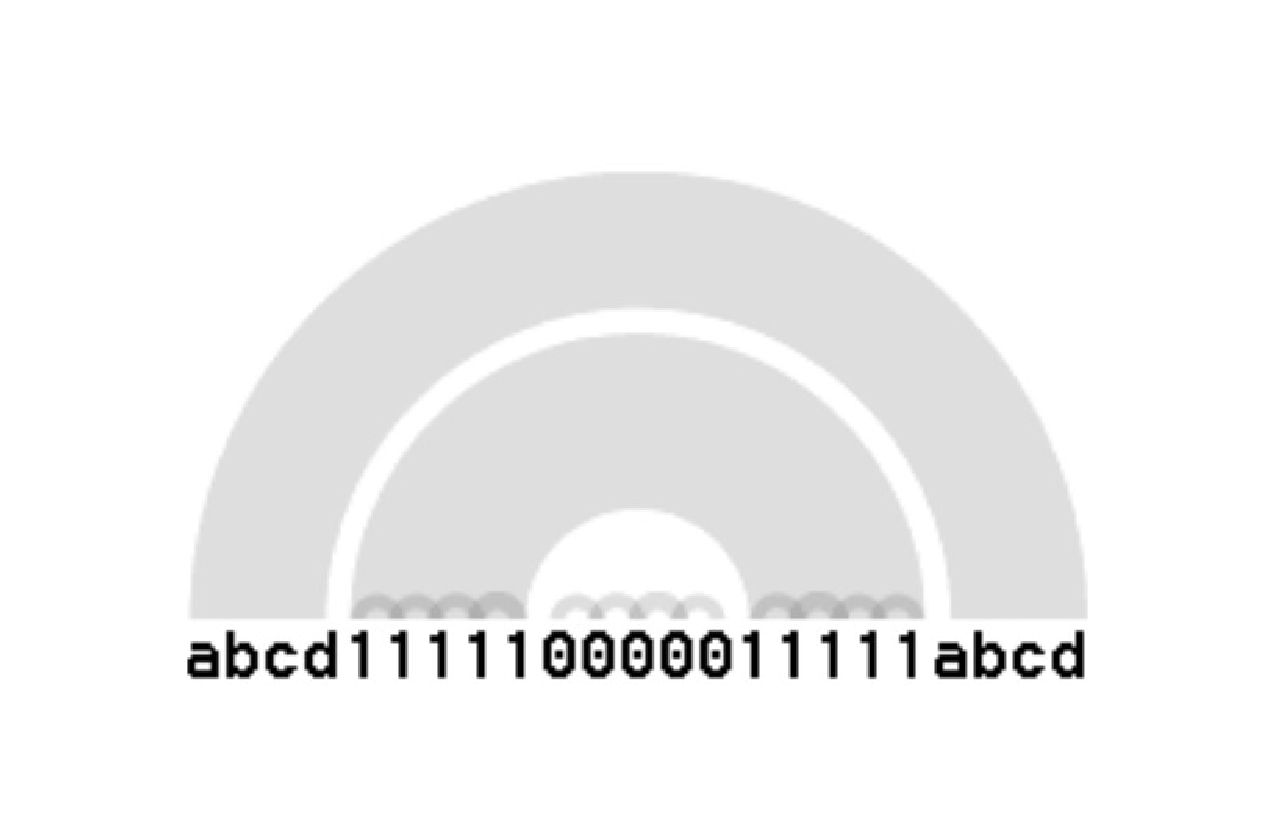
\includegraphics[width=0.9\linewidth]{arcplots.pdf}
        \caption{}
        \label{fig:genomic}
    \end{subfigure}%
    \begin{subfigure}{0.5\linewidth}
        \centering
        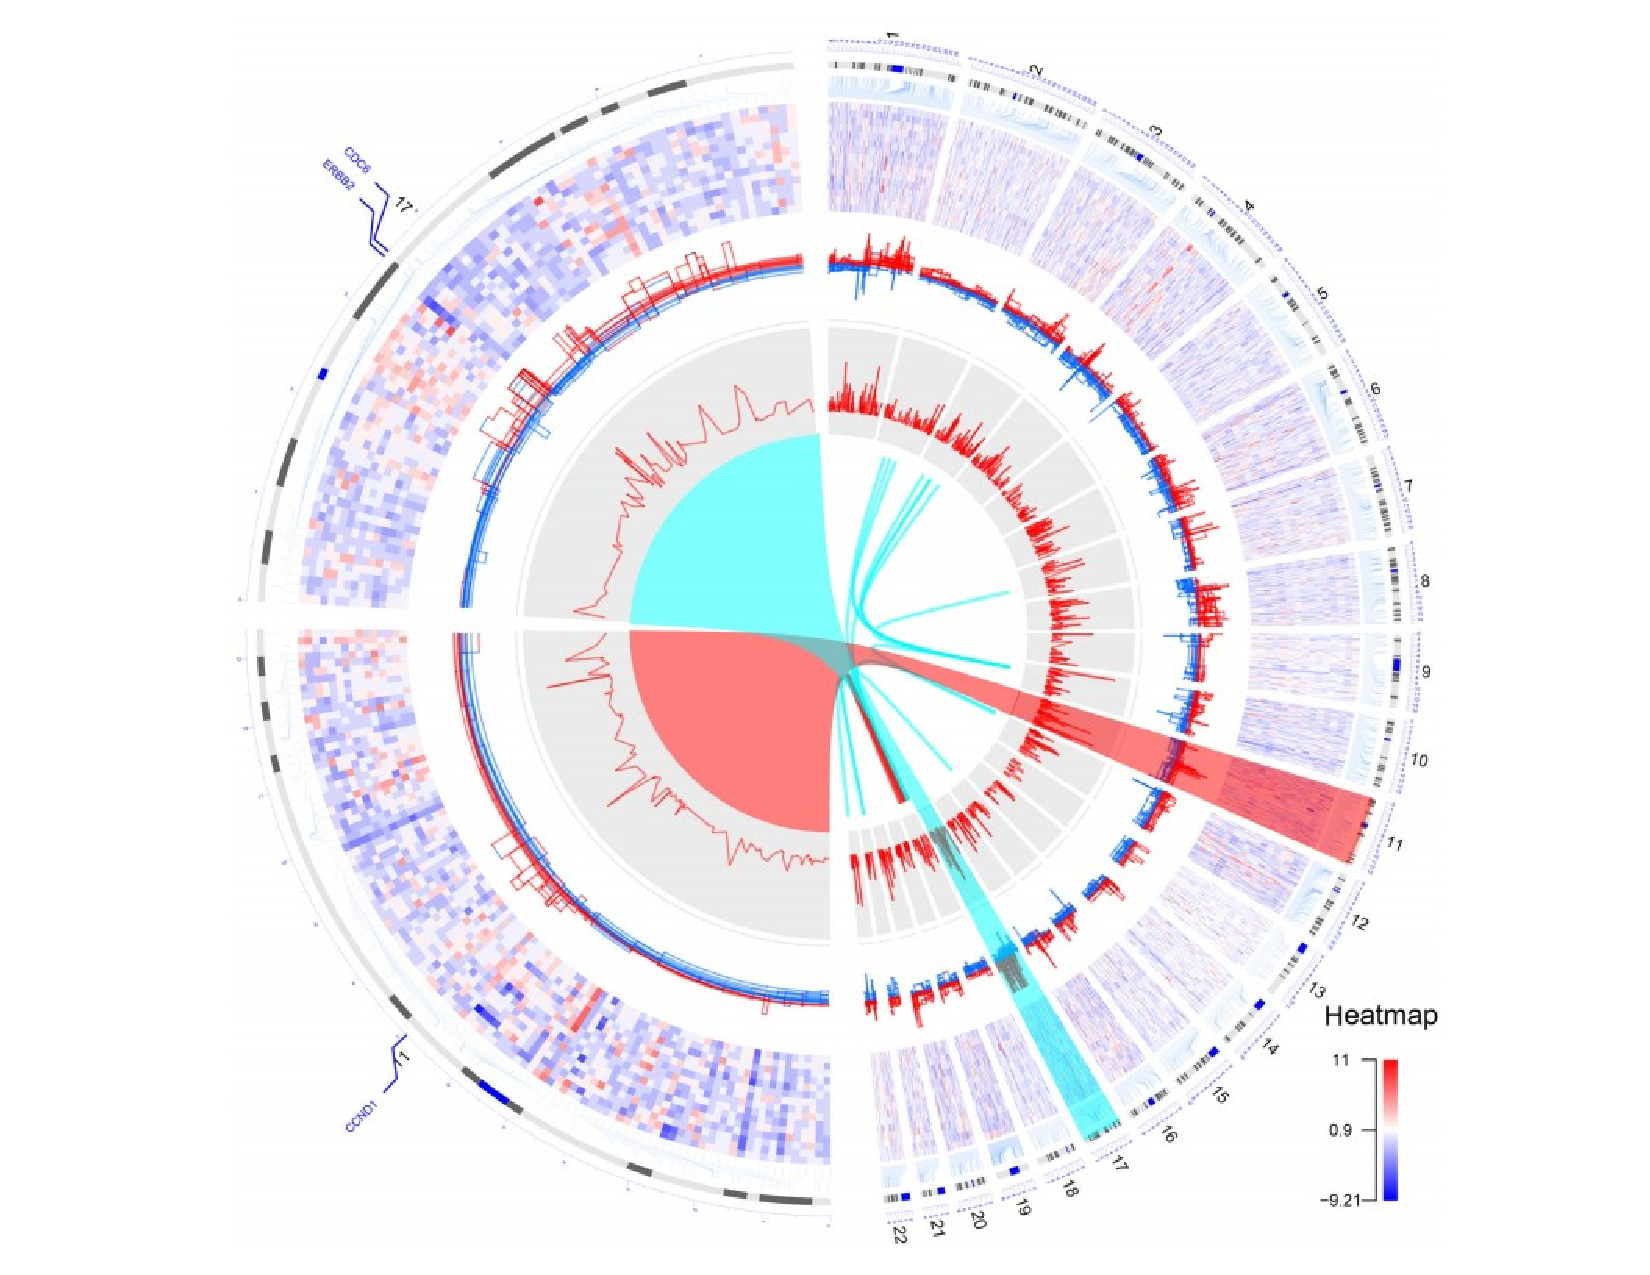
\includegraphics[width=0.9\linewidth]{genomics.pdf}
        \caption{}
        \label{fig:genomic}
    \end{subfigure}
    \caption{A - Diagram for string association. This image is taken from the works from \cite{arcplots}; B - Circular plot by OmicCircos. Several layers (Circular tracks) identify genome position, expression heatmaps, correlation between expression and CNV, among other features. The image is taken from the works from \textit{Ying Hu, et al.} \cite{genomics}.}
\end{figure}

One domain that has interesting examples in data visualization is \textit{genomics}. Graphical genome maps are found to concatenate a significant amount of information in a very compact way. Genome features and sequence characteristics are assessed with this visual strategy. An example can be found on Figure \ref{fig:genomic}. This type of visualization inspired the summarization approach proposed for time series.
\par
This visualization strategy has several elements that can be used to transform the \gls{SSM} into a compact form of filtered information. The elements are (1) multi-layered colored \textit{segments}, (2) \textit{chords} that connect to nearest neighbor \textit{segments} and (3) circular signals on top of segments. The transformation into this compact representation can be performed with the explained analysis methods above.

\subsection{A step by step example}

\begin{figure}
\centering
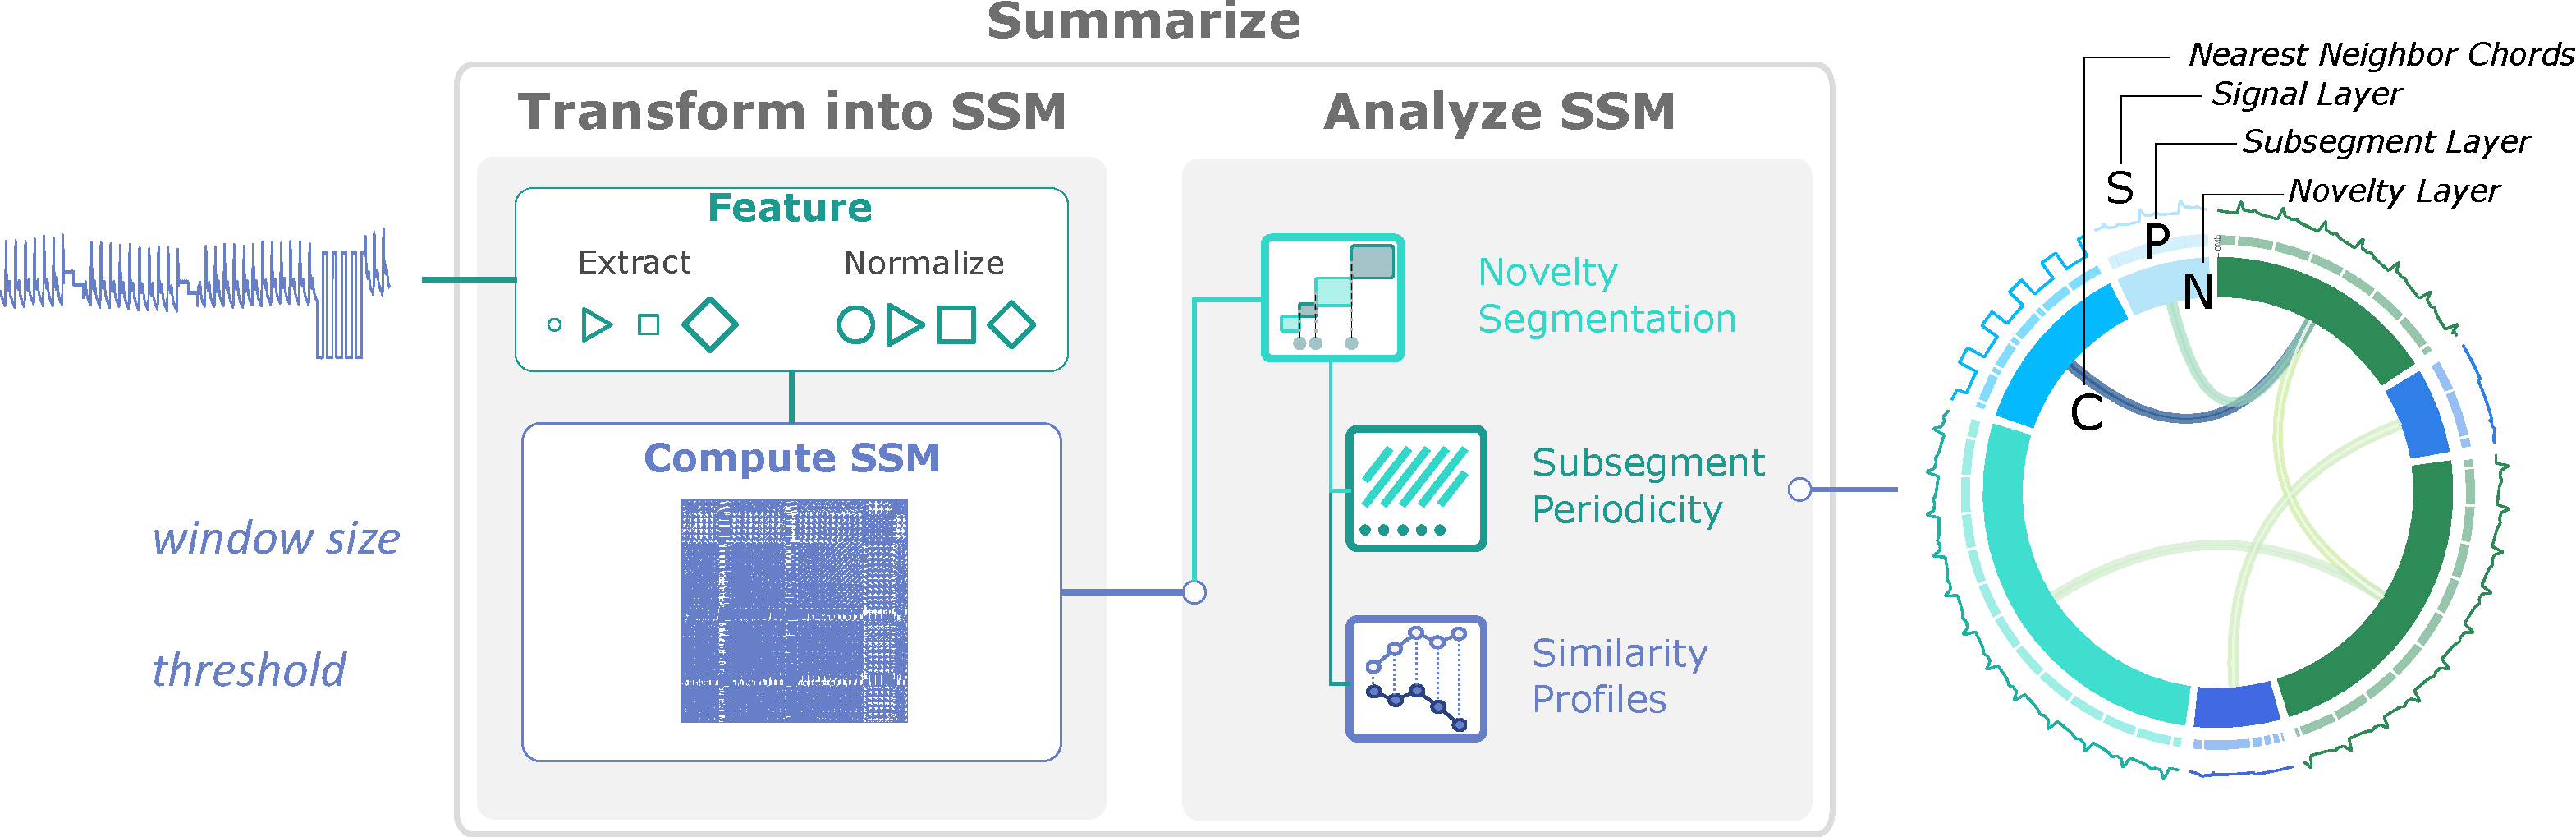
\includegraphics[width=\linewidth]{summarize_steps.pdf}
\label{fig:summarize_steps}
\end{figure}

The steps are indicated in Figure \ref{fig:summarize_steps} for the \gls{ABP} signal example. After computing the \gls{SSM}, it is firstly analyzed to segment the signal based on the \textit{nova} function. These segments are then compared based on the \textit{similarity profiles}. Additional layers can be created by performing an iterative and multi-scale segmentation. With this process, the time series is segmented (\textit{novelty layer}), subsegmented (\textit{subsegment layer}), each segment is connected to the nearest neighbor segment (\textit{nearest neighbor chords}) and the colors for each segment is given based on their similarity to the first segment. Figures \ref{fig:summarize_step1}, \ref{fig:summarize_step2} and \ref{fig:summarize_step3} show the step-by-step process to summarize the time series by analyzing the \gls{SSM}. 

\begin{figure}
\centering
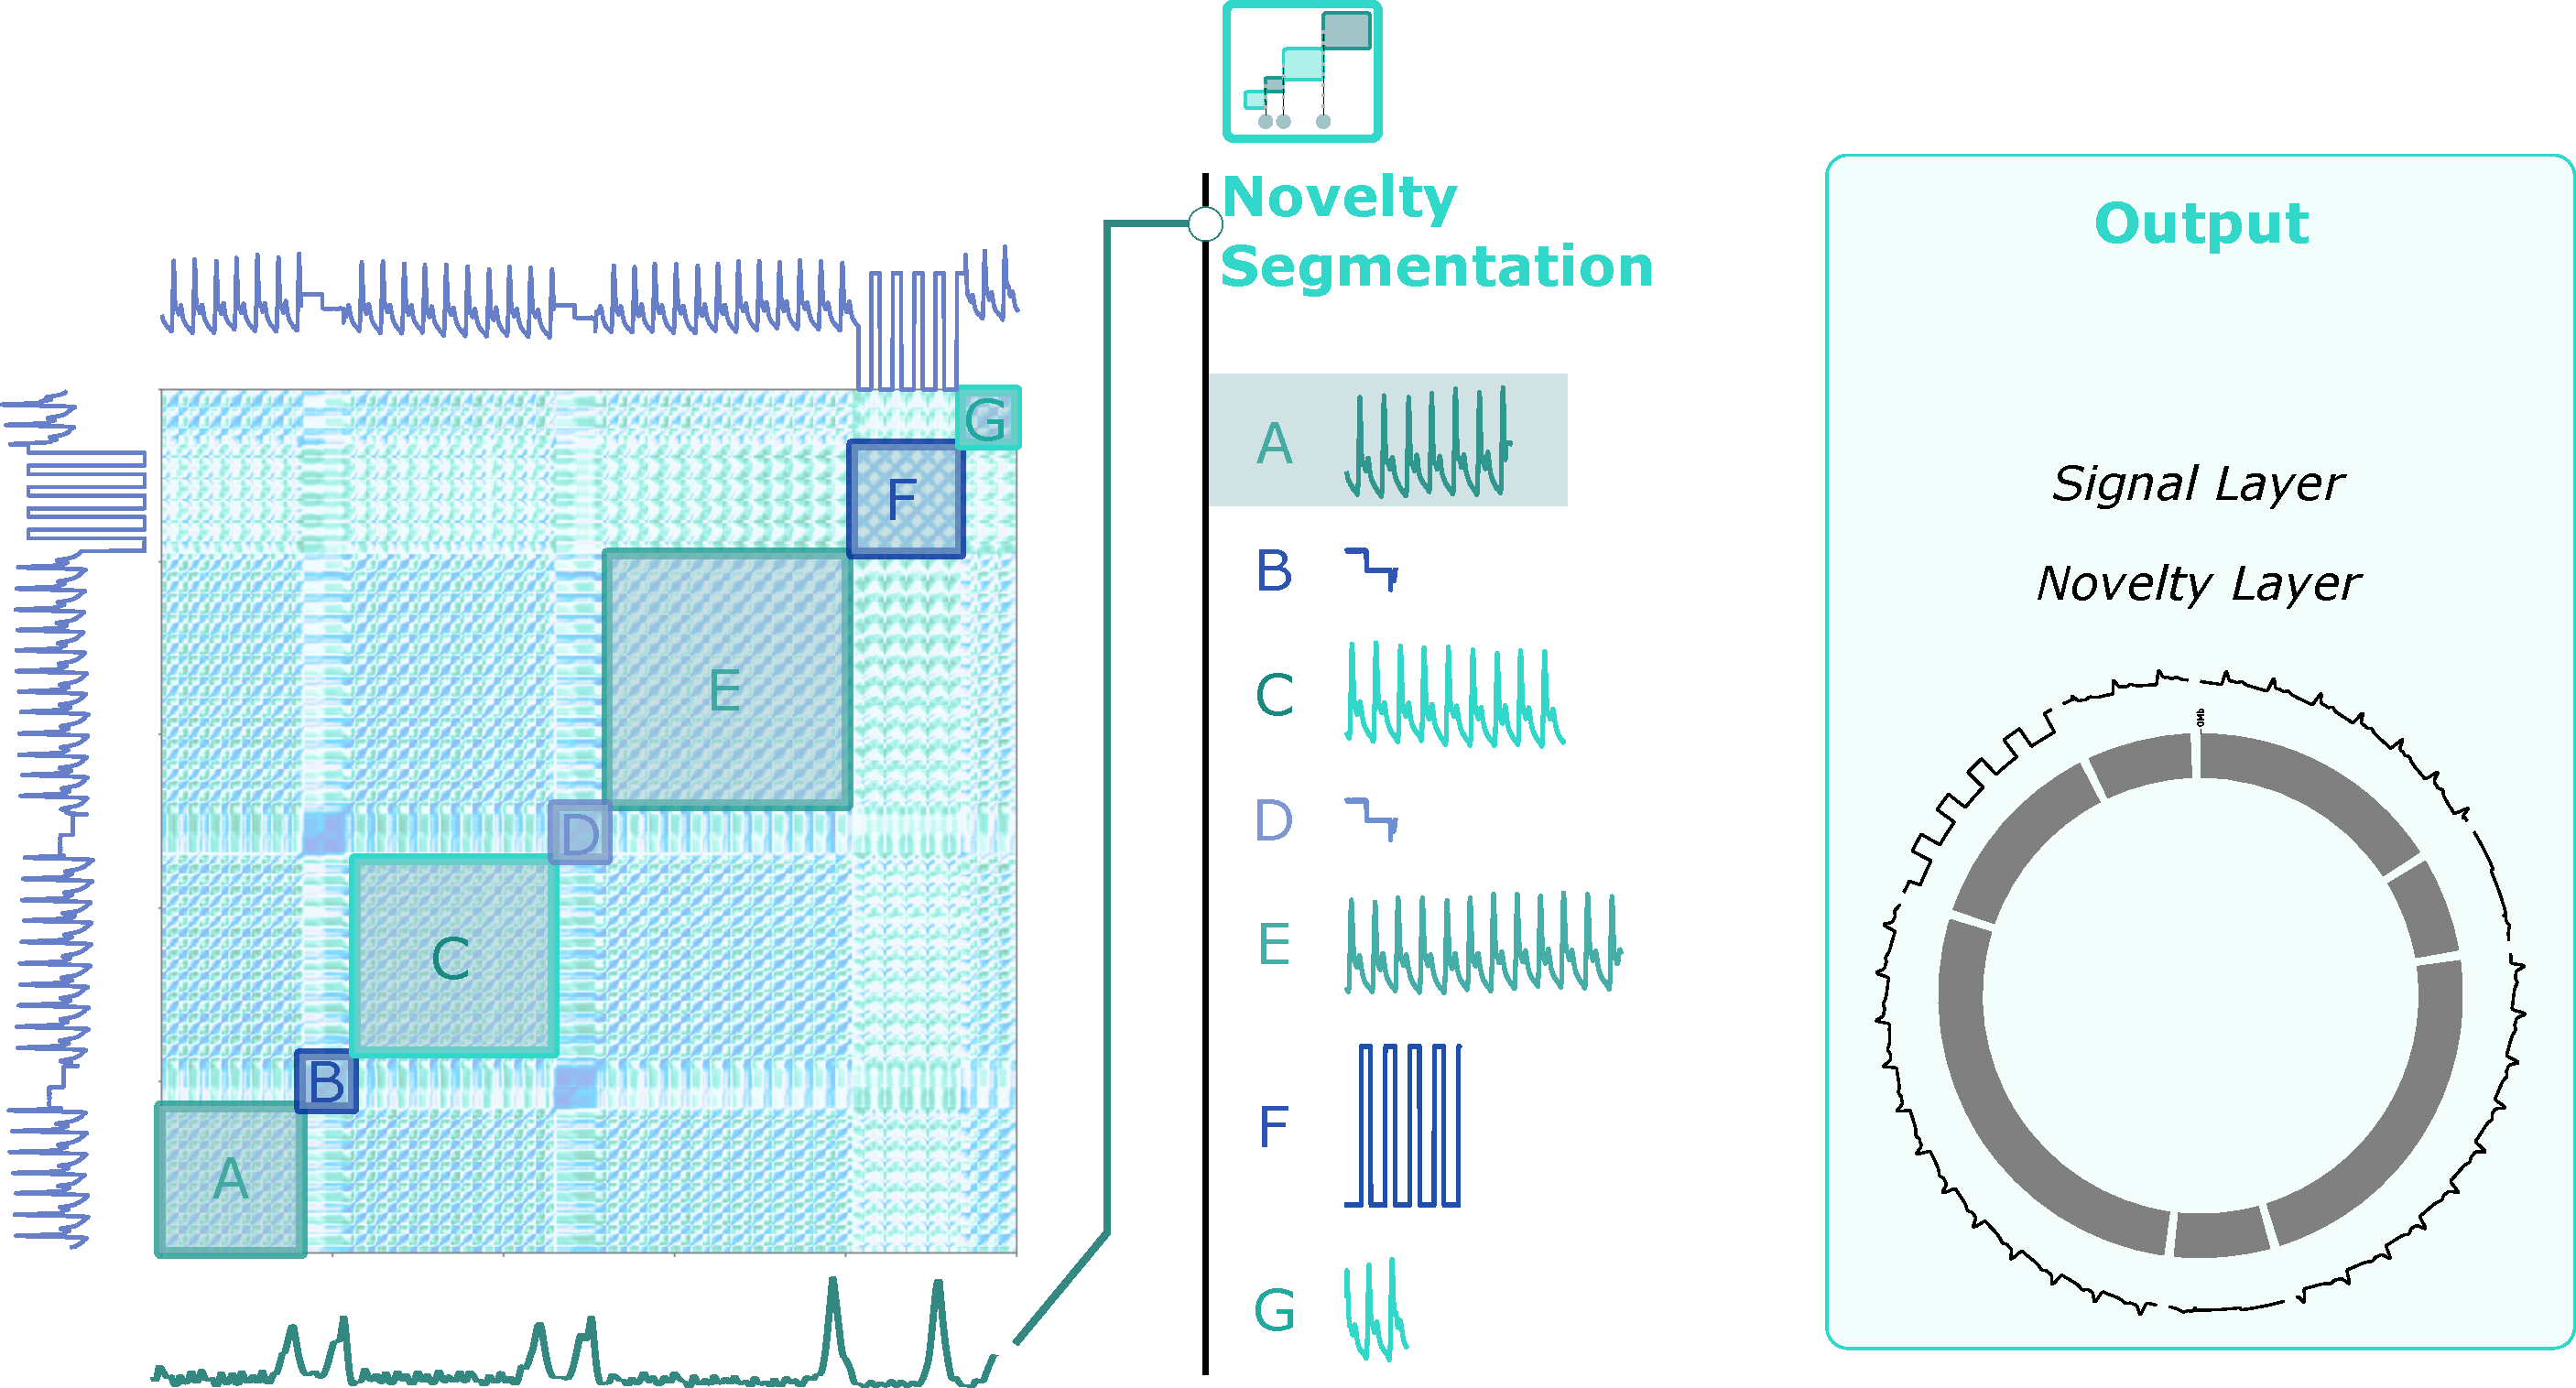
\includegraphics[width=0.85\linewidth]{summarize_step1.pdf}
\label{fig:summarize_step1}
\end{figure}

The \textit{nova} function segments the time series into seven segments. The reader can notice that segments A, C, E and G are similar and separated by segments B, C and F, represented by a failure in the connection of the sensor. From this first segmentation, the \textit{novelty layer} is created, indicating how structured is the signal, as presented in Figure \ref{fig:summarize_step1}.

\begin{figure}[b]
\centering
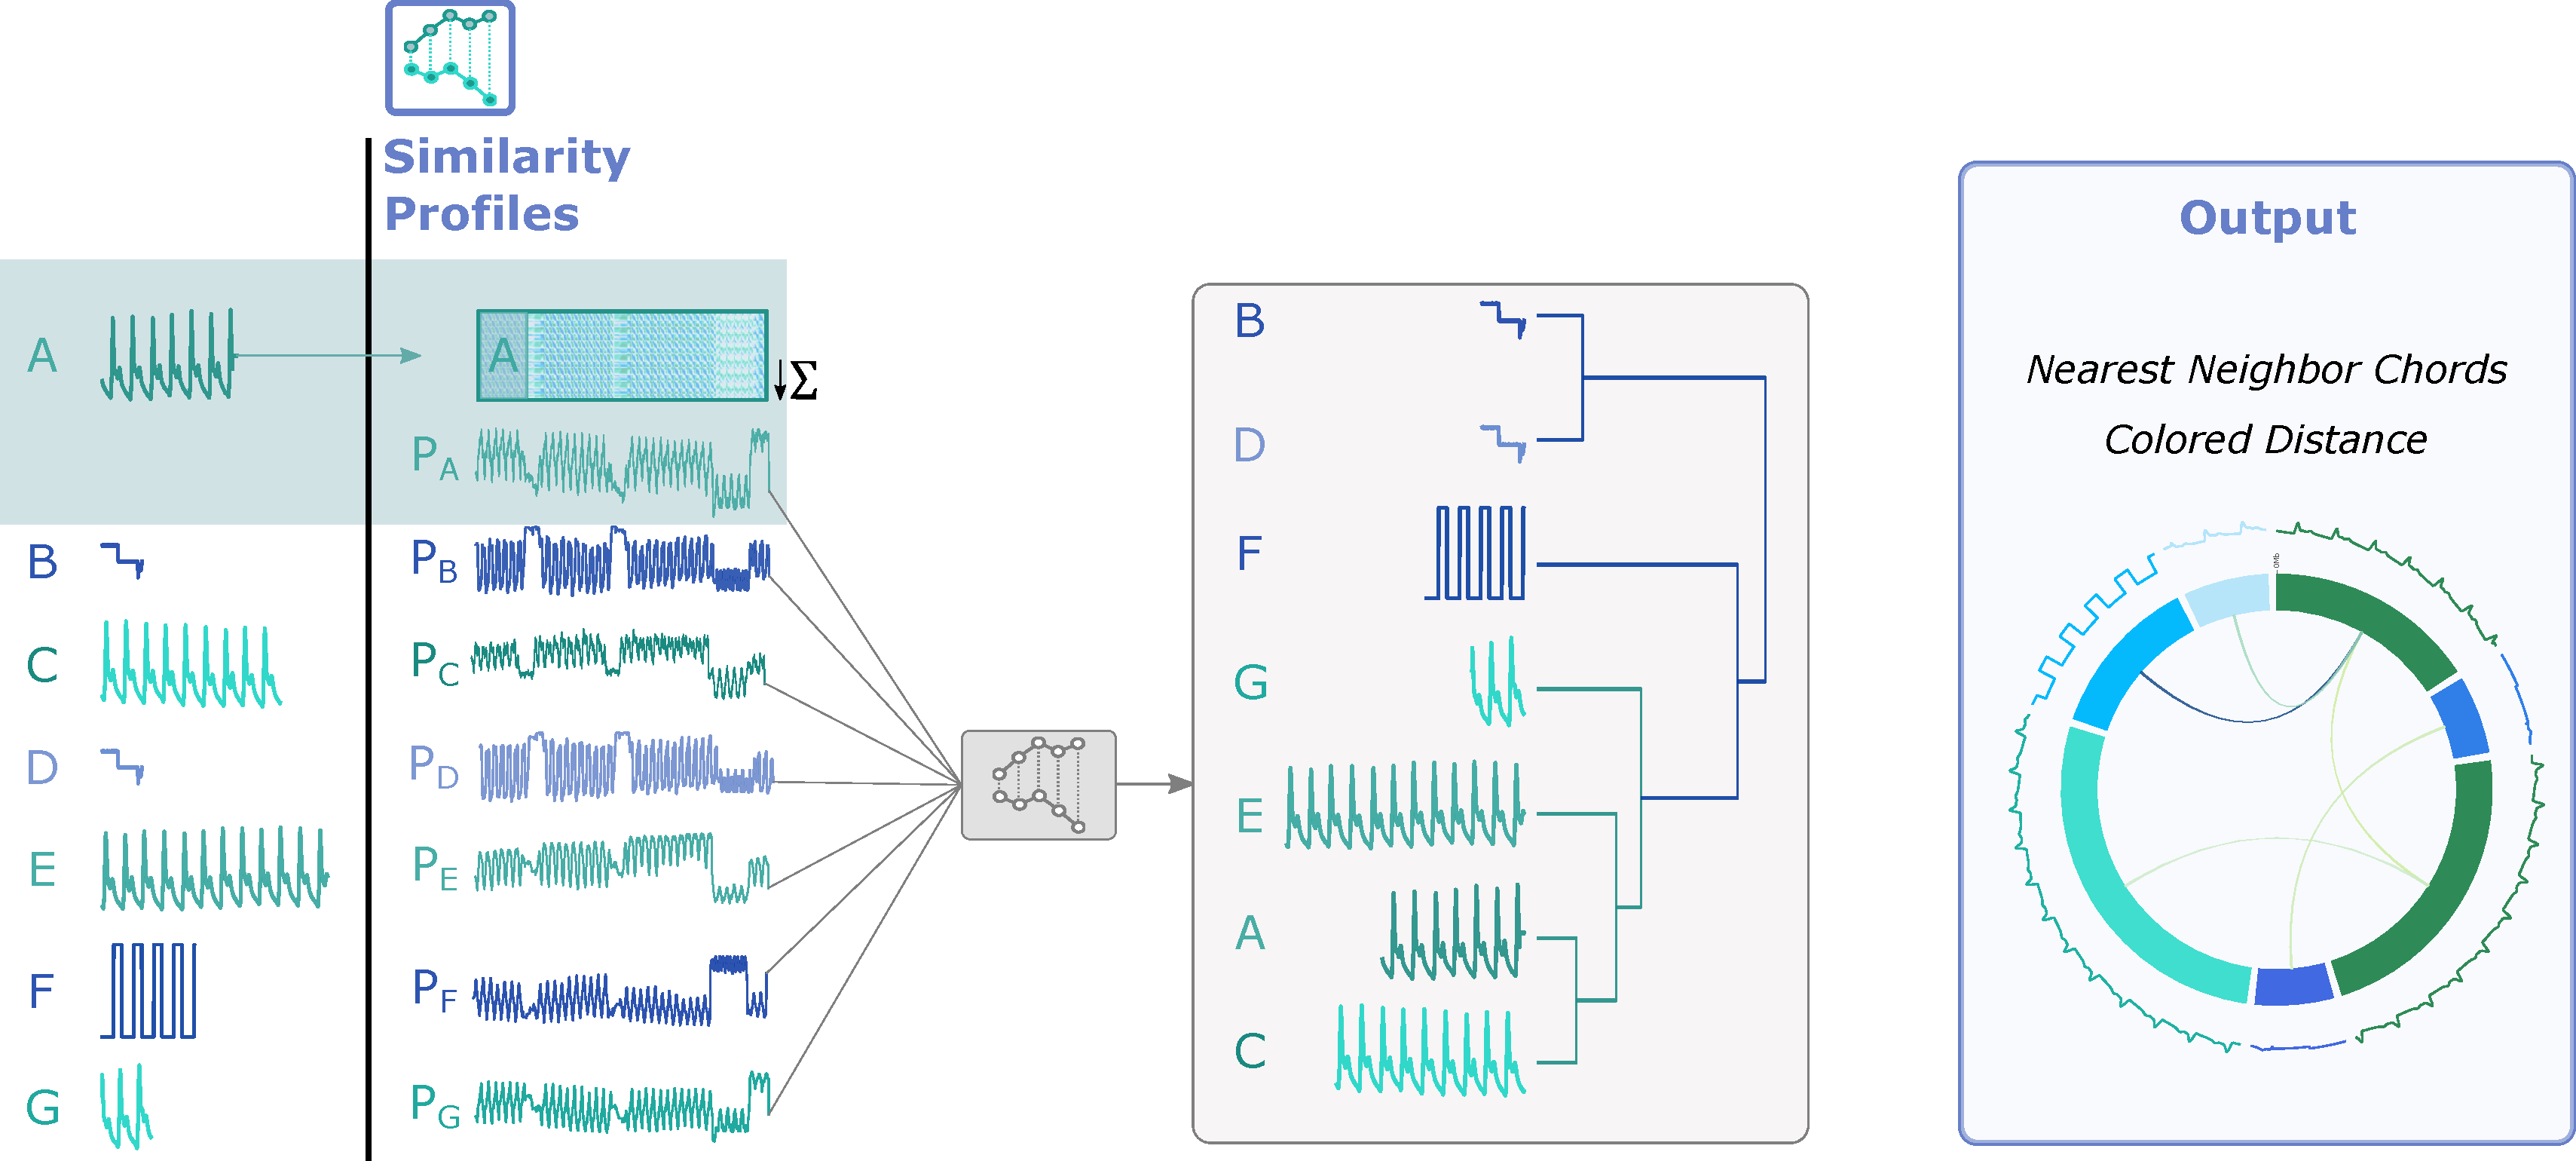
\includegraphics[width=\linewidth]{summarize_step2.pdf}
\label{fig:summarize_step2}
\end{figure}

Further, the segments are compared with the \textit{similarity profiles} of each segment. Figure \ref{fig:summarize_step2} illustrates as example the rows of the \gls{SSM} delimited by segment A and the column-wise average into $P_A$. The same process is applied to each segment. From this Figure, the reader may notice that the profiles $P_A$, $P_C$, $P_E$ and $P_G$ are more similar, while profiles $P_B$ and $P_D$ are more similar as well. The pairwise distance is computed between profiles, which can then be used to extract the nearest neighbor of each segment, as well as transform the distance values between segments into color. 
\par
The pairwise distance between profiles is also used to illustrate how the segments are ordered and clustered by the dendogram of Figure \ref{fig:summarize_step2}. The dendogram shows that there are three main clusters, being cluster one represented by segments A, C, E and G; the second cluster has segment F and the third cluster groups segments B and D. It is important to note that typical distance measures, such as the \gls{ED} or \gls{DTW}, would not be able to directly sort these segments correctly. Using \textit{similarity profiles} is more robust and invariant to the size and time distortions. 

\begin{figure}
\centering
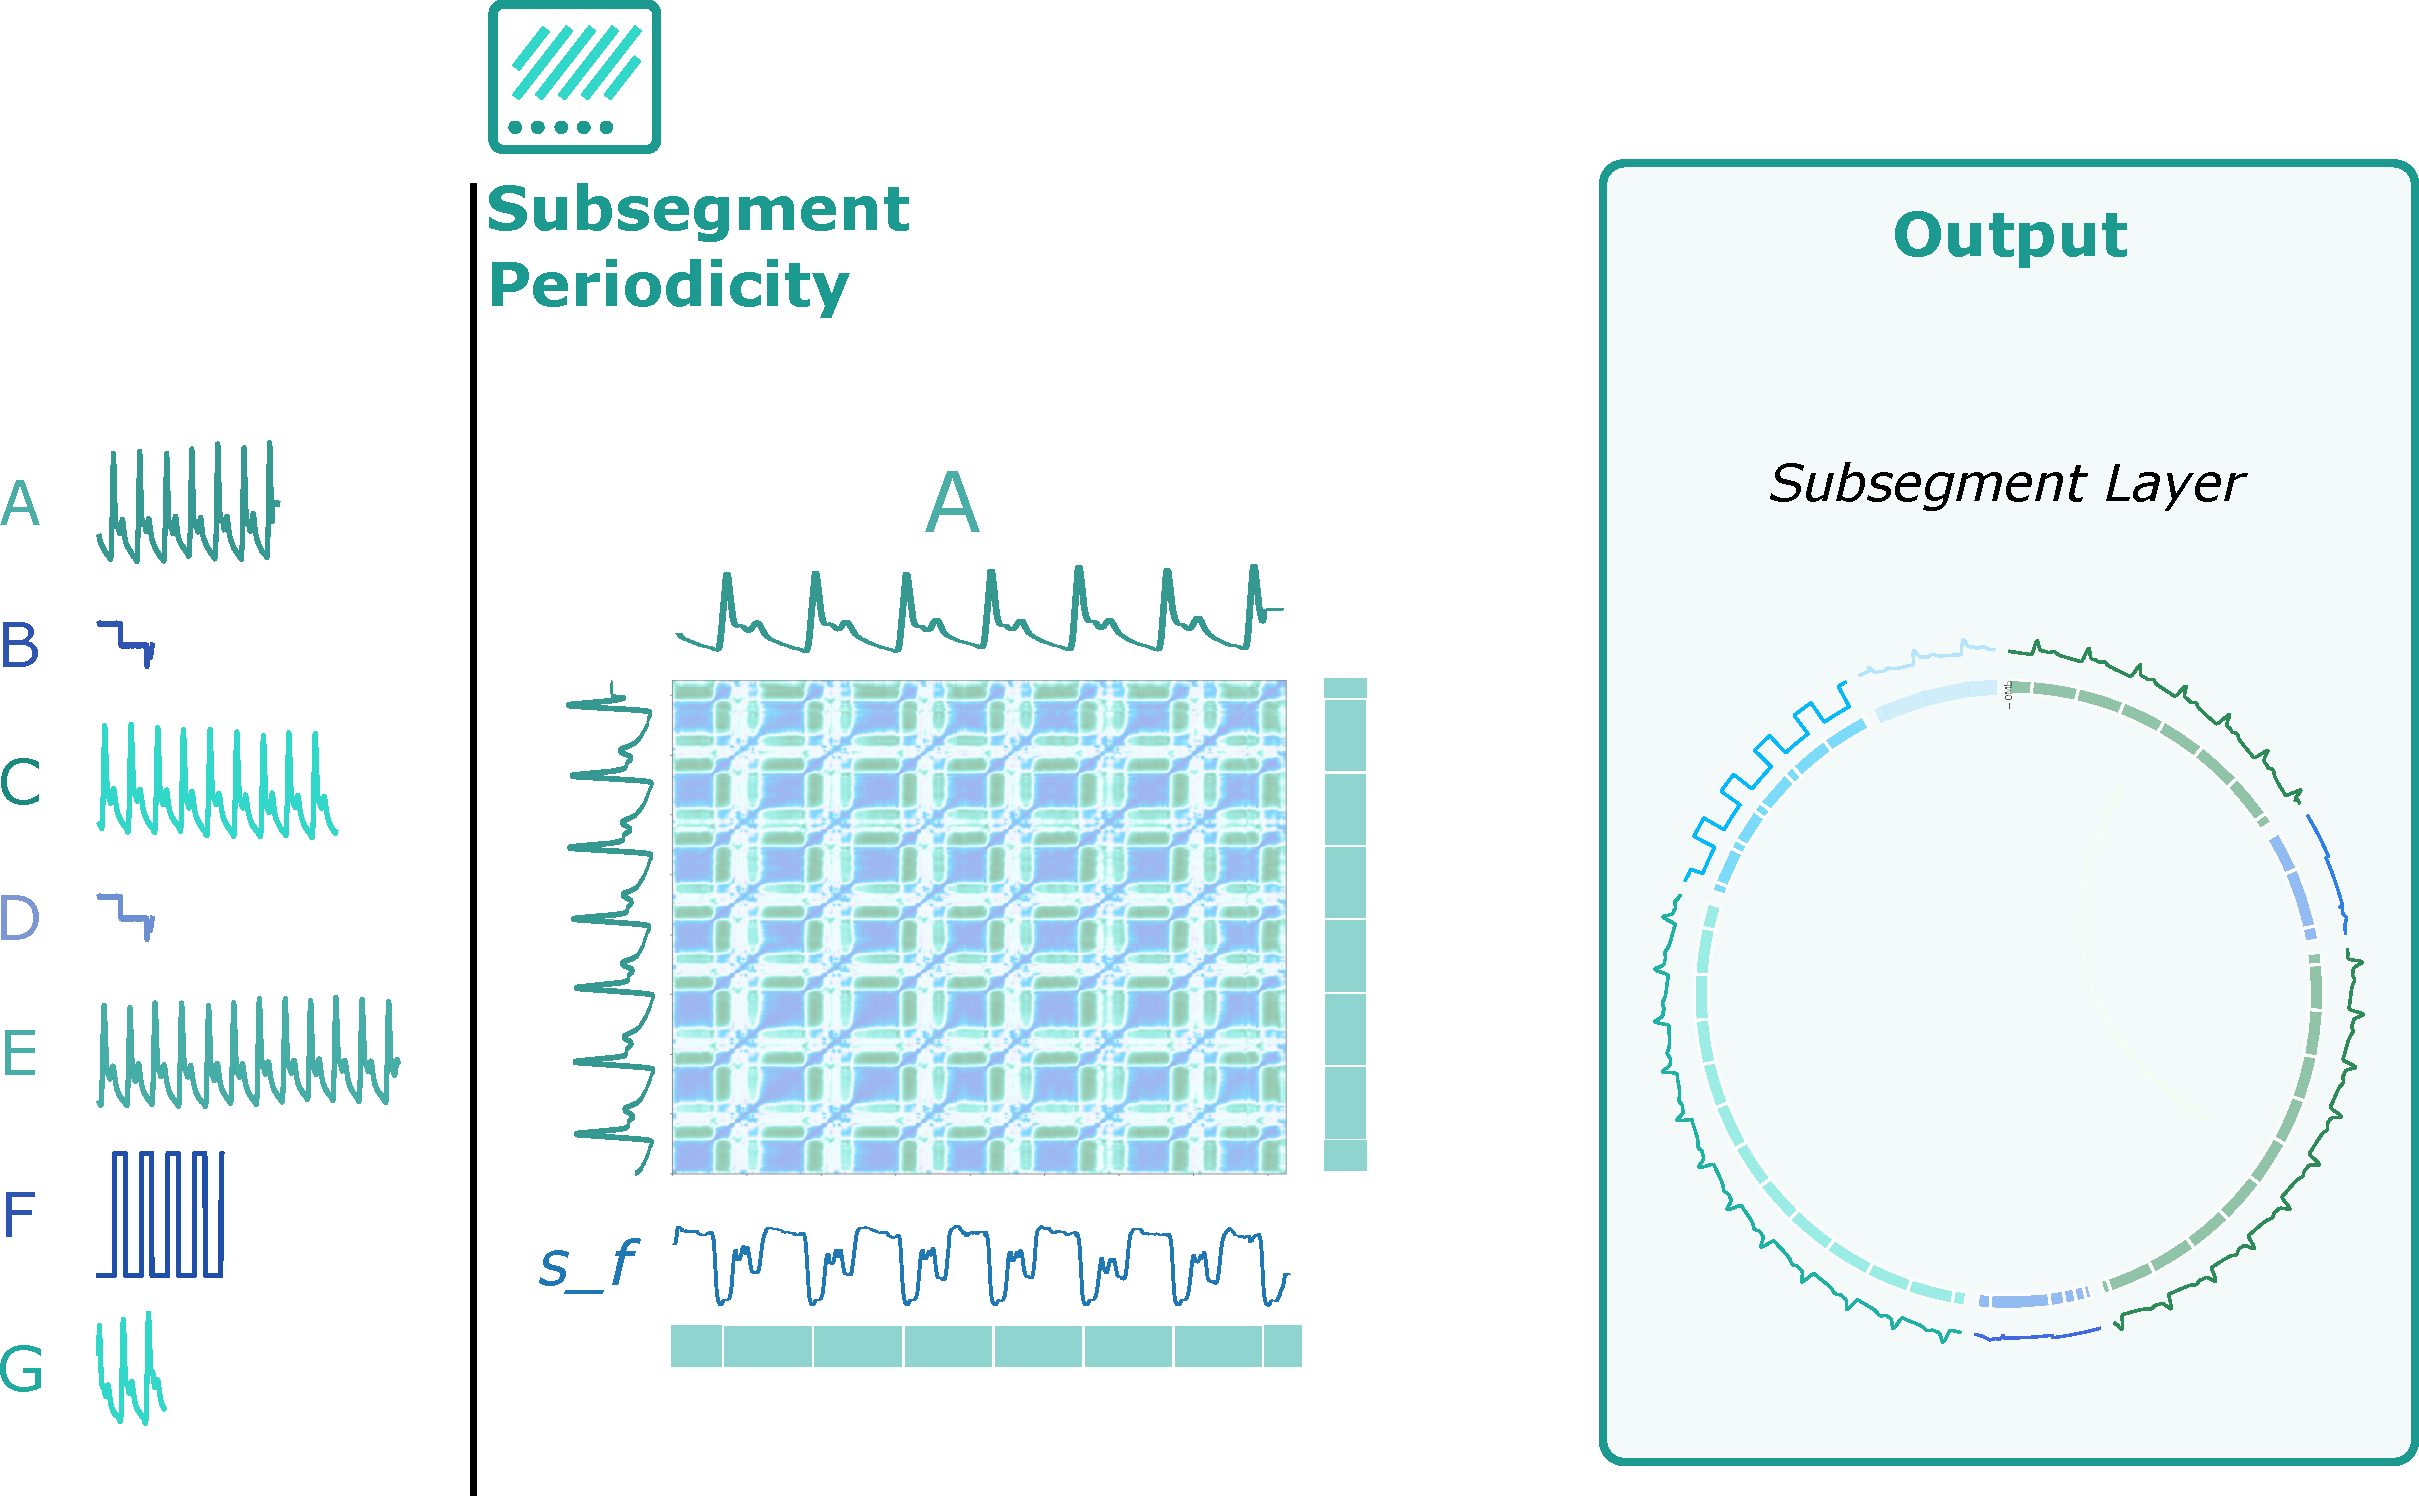
\includegraphics[width=0.75\linewidth]{summarize_step3.pdf}
\label{fig:summarize_step3}
\end{figure}

Finally, the process to summarize the time series can be iterative by adding \textit{subsegment layers}. These layers can be added by performing the \textit{novelty search} on the previously segmented time series with a smaller time scale, or segmenting the time series based on periodicity. In this case, the signal is periodic, therefore Figure \ref{fig:summarize_step3} illustrates the \textit{periodic search}, where periods are segmented by the minima of the $s_f$. 
